
\chapter{Experiments and Discussion}

\section{Introduction}
In this chapter, we perform different experiments for the following purposes:
\begin{itemize}
	\item to evaluate the performance of uncertainty estimation of dropout variational inference and its variants as well as Laplace approximation. Comparisons and analysis towards the results of these two kinds of approach are given.
	
	\item to evaluate performance of training a domain specific classifier, with different strategies for collecting training data including manual labeling and automatic labeling, where the latter one is chosen based on uncertainty estimation.
	
	\item to evaluate performance of classifier including context information via CRF.
\end{itemize}

Before looking into the results, we need to specify the details of experiments such as the dataset, evaluation metrics. Besides, the detailed parameters of the model will be reported in section of each experiment to avoid confusions. Models were implemented in Tensorflow\cite{abadi2016tensorflow}, and optimization was performed using RMSprop with initial learning rate of $1e^{-5}$ and L2 regularization with coefficient of $3.5e^{-6}$ as well dropout regularization with coefficient of $1.0e^{-5}$. We used early stopping with all methods, where the amount of epochs to run was determined based on performance on a validation set. We set the number of maximum epoch as 20.

\subsection{Dataset}
\paragraph{WRGBD\cite{lai2011large}} This dataset is a large-scale dataset of 300 household objects captured from multi-viewpoint. The objects are organized into 51 categories, some of categories and their subtrees are shown in figure \ref{fig:wrgbd1}. To note that category level recognition involves classifying objects with similar semantic appearance such as cereal boxes with different texture into same category, instead of just physical appearance. Instance level recognition is to classify objects with similar physical appearance to the same category. Therefore the overlapping of features between classes in category recognition is larger than that in instance recognition. More abstract and semantic concepts are expected to be learned in category recognition. Each object was placed on a turn table and captured from a systematically sampled view hemisphere with $15^{\circ}$ step in elevation (from $30^{\circ}$to $60^{\circ}$) and $2^\circ$ step in azimuth (from $0^\circ$ to $360^\circ$) (cf. figure \ref{fig:wrgbd2}). The total size of entire dataset is around $160.9\times10^3$. 

\begin{figure}[h!]
	\begin{center}
		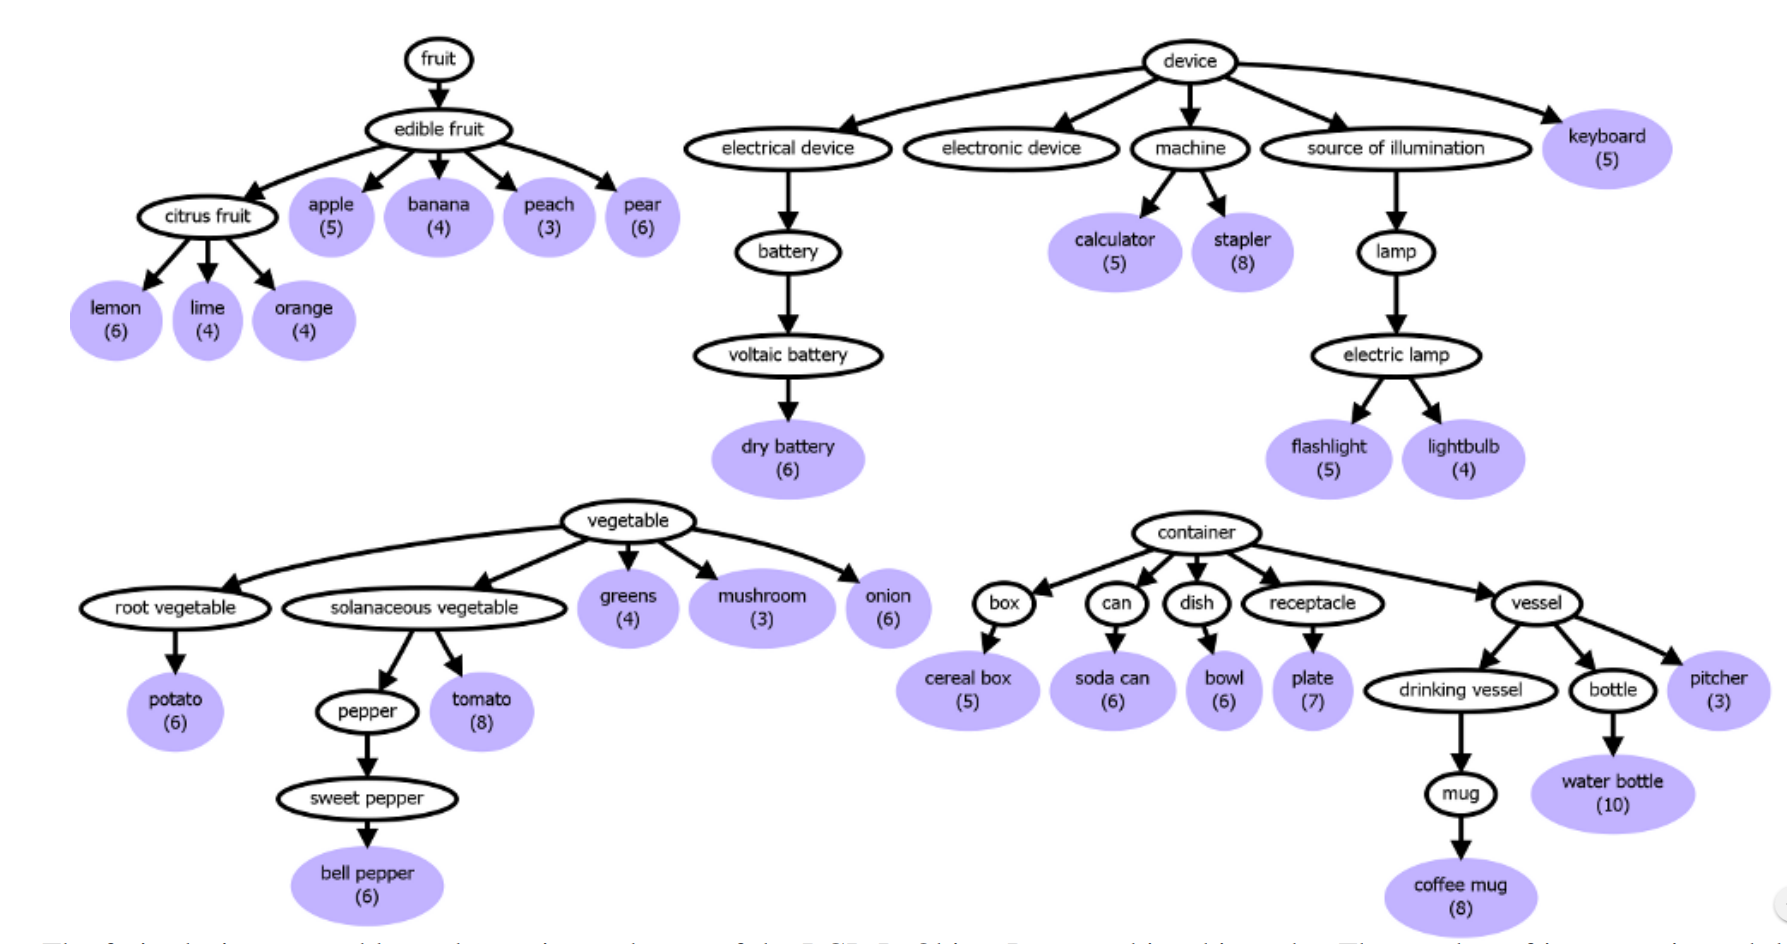
\includegraphics[height=6cm, width=13cm]{wrgbd1_}
		\caption{The fruit, device, vegetable, and container subtrees of the RGB-D Object Dataset object hierarchy, the shaded ellipse represent categories and number inside parenthesis denotes the number of instances within this category\cite{lai2011large}.}		
		\label{fig:wrgbd1}
	\end{center} 
\end{figure}
\paragraph{UniHB} To simulate application-specific situation in deployment of robots, we recorded a similar dataset by putting objects on a turn table in front of the robot and recording partial views of objects. We follow the same methodology as \cite{lai2011large} suggests for WRGBD, but with only one object instance for each category in the dataset. This analogue of WRGBD dataset is called the IAI-ODU dataset of UniHB. The size of data with elevation $45^\circ$ is around $8.6\times10^3$ and that of data with elevation $30^\circ$ and $60^\circ$ is around $17.1\times10^3$.

While the UniHB dataset's setup strives to mimic the WRGBD one, the differing capturing conditions such as different equipment and light conditions even appearances of objects, result in obvious changes in feature space, thus yielding a significant drop on classification accuracy. In addition to the existing 51 categories, there are 28 novel objects(cf. figure \ref{fig:not_in_wrgbd}) that do not belong to the 51 categories and these objects are treated as out-of-distribution(OOD) data for testing uncertainty estimation of the model. To note that data of these novel objects are recorded in a slight different way, that is, their view points are sampled with $15^{\circ}$ step in elevation (from $30^{\circ}$to $60^{\circ}$) and $5^\circ$ step in azimuth (from $0^\circ$ to $360^\circ$). The size of this OOD dataset is around $6.0\times10^3$.


 \begin{figure}[H]
 	\begin{center}
 		\includegraphics[height=10cm, width=16cm]{domain_diff}
 		\caption{Example of masked images of objects from 51 categories in WRGBD and UniHB dataset. In each category, the left is from WRGBD and the right is from UniHB. We randomly pick one instance for the objects of WRGBD. We can see some light and appearance difference between objects in these two datasets.}		
 		\label{fig:wrgbd2}
 	\end{center}
 \end{figure}

\begin{figure}[H]
	\begin{center}
		\includegraphics[height=7cm, width=12.5cm]{not_in_wrgbd}
		\caption{Example of masked images of objects from 28 categories which are not belonging to WRGBD categories, which are treated as OOD data samples.}		
		\label{fig:not_in_wrgbd}
	\end{center}
\end{figure} 

\paragraph{T-LESS\cite{hodan2017tless}}


\subsection{Uncertainty measures}
For each prediction, we can obtain one predictive probability distribution from our model with equation \ref{marginalization_test}. In order to quantify uncertainty of the prediction, there are different metrics to measure the uncertainty of prediction, which are introduced in the following. We define $x^\star$ as one test data sample and $\mathcal D$ as our training set. 
\paragraph{Confidence} is defined as the maximum probability of the output predictive distribution, whose index is the class prediction.

\begin{equation}\label{confidence}	
\begin{aligned}
conf = \max_c \big[ p(y=c|x^\star, \mathcal D) \big]
\end{aligned}
\end{equation}
where $conf \in [0,1]$, $c \in \mathcal P = \{0,...,|\mathcal P|-1\}$, and $\mathcal P$ represents output space in which label is expressed as number index which is transformed into one-hot representation in computation of objective function. The larger this quantity is, the less uncertain the prediction is. 

\paragraph{Predictive entropy} is quantity that captures the average amount information contained in predictive distribution\cite{shannon1948mathematical}: 
\begin{equation}\label{entropy}	
\begin{aligned}
\mathcal H[p(y|x^\star, \mathcal D)] = -\sum_{c}p(y=c|x^\star, \mathcal D)\text{log}p(y=c|x^\star, \mathcal D)
\end{aligned}
\end{equation}
where $c$ is the possible class $y$ can take, $\mathcal H(\cdot) \in [0, \text{log}{|\mathcal P|}]$, the larger this quantity is, the more uncertain the prediction is.

\paragraph{Mutual information}
Mutual information between the prediction $y$ and the weights posterior offers a different uncertainty measure when compared with the aforementioned ones. This measure is widely used in active learning tasks\cite{houlsby2011bayesian}, which is also called Bayesian active learning disagreement(BALD). The definition of this measure is as follows:
\begin{equation}\label{mi}	
\begin{aligned}
\mathcal I[y,\bld \omega|x^\star, \mathcal D] &= \mathcal H[y|x^\star, \mathcal D] - \mathbb E_{p(\bld \omega| \mathcal D)}\big[\mathcal H[y|x^\star, \bld \omega] \big] \\
&= -\sum_{c}p(y=c|x^\star, \mathcal D)\text{log}p(y=c|x^\star, \mathcal D) \\ &+ \mathbb E_{p(\bld \omega|\mathcal D)}[-\sum_{c}p(y=c|x^\star, \bld \omega)\text{log}p(y=c|x^\star, \bld \omega)] \\
&\approx -\sum_{c}p(y=c|x^\star, \mathcal D)\text{log}p(y=c|x^\star, \mathcal D) \\ &+ \mathbb E_{q(\bld \omega)}[-\sum_{c}p(y=c|x^\star, \bld \omega)\text{log}p(y=c|x^\star, \bld \omega)]
\end{aligned}
\end{equation}
where $\mathcal I(\cdot) \in [0,\text{log}{|\mathcal P|}]$.
This quantity considers the effect of approximate posterior distribution more directly. Compared with aforementioned uncertainty measures, this one should be able to capture the model uncertainty more accurately. To think about it intuitively, this quantity measures the information gain between the entropy of predictive output distribution and the expected entropy of output distribution wr.t. weights posterior. It will be low only if the predictive distribution agrees with most of possible models(weights realizations), which means that the model is sure about its prediction. Otherwise, it will be high because most of possible models do not agree with the other models and thus the predictive distribution will be more uniform and thus has higher entropy.

\subsection{Evaluation metrics}
As is stated in \cite{gneiting2007probabilistic}, the goal of probabilistic prediction is to maximize the sharpness of predictive distribution subject to calibration. Calibration refers to the statistical consistency between the predictive probability and the occurrence of observations, which is the frequency of the event. Therefore we employ different metrics including both the accuracy and other quantities related to calibration as well as summary of accuracy and calibration. Additionally, we also employ histogram and diagram to express the results visually. While the visual one can show us the results more intuitively, the quantitative one can allow us to evaluate the results more objectively. The comparison between them may help us to examine if visual metrics are corresponding to the numerical metrics, which may provide more insights in evaluating uncertainty estimation. 

\paragraph{Uncertainty histogram} is a intuitive visual tool for analyzing the statistics of the uncertainty estimation. Compared with normal histogram, there is one difference to stress on. In order to make visual effect more clear and hence the analysis easier, \textbf{normalizer} of each type of prediction is the size of this type of predictions instead of size of all predictions. In detail, we have three types of prediction for plotting the histogram, which are:
 \begin{itemize}
 	\item \textbf{correct prediction}
 	\item \textbf{miss-classification}
 	\item \textbf{out-of-distribution(OOD)}
 \end{itemize}The range of y axis is $[0,1]$ because we normalize the number in each bin, and range of x axis is set by the range of corresponding type of uncertainty measure.

\paragraph{Reliability diagram(Calibration curve)} is another visual tool for expressing \textbf{calibration} performance of the model\cite{guo2017calibration}, which plots the frequency of success(accuracy of predictions in specific bin) as a function of confidence, which is predictive likelihood of prediction. If the model is perfectly calibrated, this function should be overlapping with the diagonal line exactly. The closer this curve is to diagonal curve, the better the calibration performance is. In order to draw the curve, we firstly group the predictions into $M$ interval bins w.r.t. confidence and then calculate the accuracy of predictions in each bin. We use $M=20$ in this work. To quantify the proximity to the diagonal curve, we use two metrics:
\begin{itemize}
	\item \textbf{Expectation calibration error(ECE)}: in order to obtain a more objective measure of calibration quality, we can compute the \textbf{expected calibration error} by computing the weighted average of difference between accuracy and confidence:
	
	\begin{equation}
	ECE = \sum_{m=1}^{M}\frac{|B_m|}{n}|acc(B_m) - conf(B_m)|
	\end{equation}
	where $n$ is the number of samples, and $acc(B_m)$ represents the accuracy of samples, $conf(B_m)$ the average predicted confidence of samples in $m$-th bin. We can see that this metric measures the inconsistency between the statistics and predictive distribution. To note that this metric only considers the calibration quality instead of accuracy. One drawback of this metric is that, because the weights are computed based on number of samples in each bin, the metric would bias if most of predictions are clustering in few bins. Then the weights of these bins are much larger than other bins and other bins with large error would be ignored. 
	
	\item \textbf{Maximal calibration error(MCE)}:
	Considering the drawback mentioned in ECE, we make use of this metric. Additionally, in high risk applications where reliable confidence measures are absolutely necessary, we may wish to take the worst case into account. It is defined as follows:
	
	\begin{equation}
	MCE = \max_m|acc(B_m) - conf(B_m)|
	\end{equation}
\end{itemize}


\paragraph{Proper scoring rules:} 
Scoring rules provides a \textbf{summary} measure in the evaluation of probabilistic forecasts. It assigns a numerical score based on the difference between predictive distribution and real distribution. 

Because we want to make predictions for the future and also have a suitable measure of the uncertainty associated with them (see \cite{gneiting2007strictly} for a review). We can define the scoring rule as a function $\mathcal S(p(y|\bld x), (y|\bld x))$ that evaluates the quality of predictive distribution $p(y|\bld x)$ relative to an event $y|\bld x \sim q(y|\bld x)$ where $q(y|\bld x)$ represents the true distribution over $(y|\bld x)$. Consequently, the expected scoring rule is:

\begin{equation}\label{scoring rule}
	\mathcal S(p, q) = \int q(y| \bld x) \mathcal S(p,(y|\bld x))dy
\end{equation}

$\mathcal S(p,q)$ is proper if $\mathcal S(p,q) \leq S(q,q)$, with equality holds if and only if $p(y|\bld x) = q(y|\bld x)$. Here we adopt two simple and famous proper scoring rules in which the less it is, the better the performance is:
\begin{itemize}
	\item \textbf{averaged negative log likelihood(NLL)}:NLL is a popular metric for evaluating predictive uncertainty	\cite{quinonero2005evaluating}. This metric considers aforementioned confidence as likelihood. The smaller this metric is, the better the predictive distribution is.
	
	\begin{equation} \label{nll}
		NLL = -\frac{1}{|\mathcal D_{test}|}\sum_{i=1}^{|\mathcal D_{test}|}\text{log}(p(y_i = c_i|\bld x_i))
	\end{equation}
	where $c_i$ is the ground truth label for $\bld x_i$.	
	\item \textbf{Brier score} is the mean squared error between the target distribution(one-hot encoding label) and predictive distribution:
	
	\begin{equation} \label{bs}
	BS = -\frac{1}{|\mathcal D_{test}|}\sum_{i=1}^{|\mathcal D_{test}|}(\bld y^{gt}_i - p(\bld y_i|\bld x_i))^2
	\end{equation}
	where $\bld y^{gt}_i$ is the one-hot encoding ground truth label for $\bld x_i$. 
	
\end{itemize}

\paragraph{Separability metrics:} In addition to the summary metrics of predictive probability. We are also interested in the separability between different types of predictions, which can assist the down-stream tasks if they are highly separable (e.g. separate correct predictions and false predictions or out-of-distribution data to improve robustness of system and provide more safety guarantee). To note that, we treat the correct predictions as positive samples in the two following metrics.
\begin{itemize}
	\item \textbf{Area under Receiver Operating Characteristic curve(AUROC)}:Since one of our goals is to choose automatically labeled data based on uncertainty estimation, it's necessary to evaluate the separability between correct predictions and false predictions or out-of distribution data predictions. ROC curve describes the relationship between true positive rate($tpr=\frac{tp}{tp+fn}$) and false positive rate($fpr=\frac{fp}{fp+tn}$). Moreover, AUROC can be interpreted as the probability that a positive samples has a greater score than a negative samples. However, the drawback of AUROC is that, the normalizers of two kinds of rate in ROC curve are independent to each other. When these two normalizers differs too much. AUROC can provide misleading conclusion. For example, if the number of negative predictions is much higher than positive one, the AUROC could still achieve a relatively high value, while in fact there are already many false positives. 
	
	\item \textbf{Area under Precision Recall curve(AUPR)}: Considering the downside of AUROC, another evaluation metric is employed, that is AUPR. AUPR describes the relationship between precision($pr = \frac{tp}{tp+fp}$) and recall($tpr=\frac{tp}{tp+fn}$), which resolves the problem of different base number. In the previously mentioned case, though the AUROC is high, the AUPR will be low because the precision is low. 
\end{itemize}


\section{Uncertainty estimation experiments}

\subsection{Experiments \RNum{1}}
In this experiments, we want to evaluate our model on a relatively easy task which is instance recognition at first. That means, the appearances of different classes as well as the out-of-distribution data are highly discriminable. To this end, we separate WRGBD dataset into two subsets based on the instance class. Subset \RNum{1} contains objects with instance class from 0 to 199 (assuming that here we use index to denote the instance label) and Subset \RNum{2} contains objects with instance class from 200 to 299. 

We train our model with objects captured in elevation $30^\circ$ and $60^\circ$ of Subset \RNum{1} (in which we split off 20\% of training set as validation set for model selection in training). The size of training set and validation set is around $71.0\times10^3$. Then we test the model on objects captured in elevation $45^\circ$ of both Subset \RNum{1} and Subset \RNum{2}. In this experiment, the objects in Subset \RNum{2} serve as out-of-distribution samples because they are not present during training. The size of test set is around $35.6\times10^3$ and that of OOD dataset is around $17.8\times10^3$. 

In this experiment, we just want to test and compare the performance of different approaches. Because the OOD data is highly different to the training set. The model should express high uncertainty when facing these data. Nevertheless, the miss-classifications should have higher uncertainty than the correct predictions because the model should be confident when it makes predictions correctly. Otherwise the model is overconfident when it's confident with its incorrect predictions, which can induce hazardous consequence in some safety-critical applications. As we can see in the figure \ref{exp1_histo}, the original ResNet50 model is highly overconfident, which assigns high confidence to nearly $50\%$ of miss-classification and nearly $30\%$ of OOD data in the highest bin. While the model with concrete dropout and multi-drop can significantly decrease these two proportions. As we can see, different uncertainty show similar trend in this experiment.

In addition to uncertainty histogram, we also plot the calibration curve of each model evaluated on both test set and OOD dataset in figure \ref{exp1_reliability}. As expected, the calibration performance of original model is much worse than those of the other two models. This result is corresponding to the results in \cite{guo2017calibration}, that the model is highly overconfident. And the concrete dropout and multi-dropout can mitigate the undesired problem significantly.

\begin{figure}[H]
	\begin{center}
		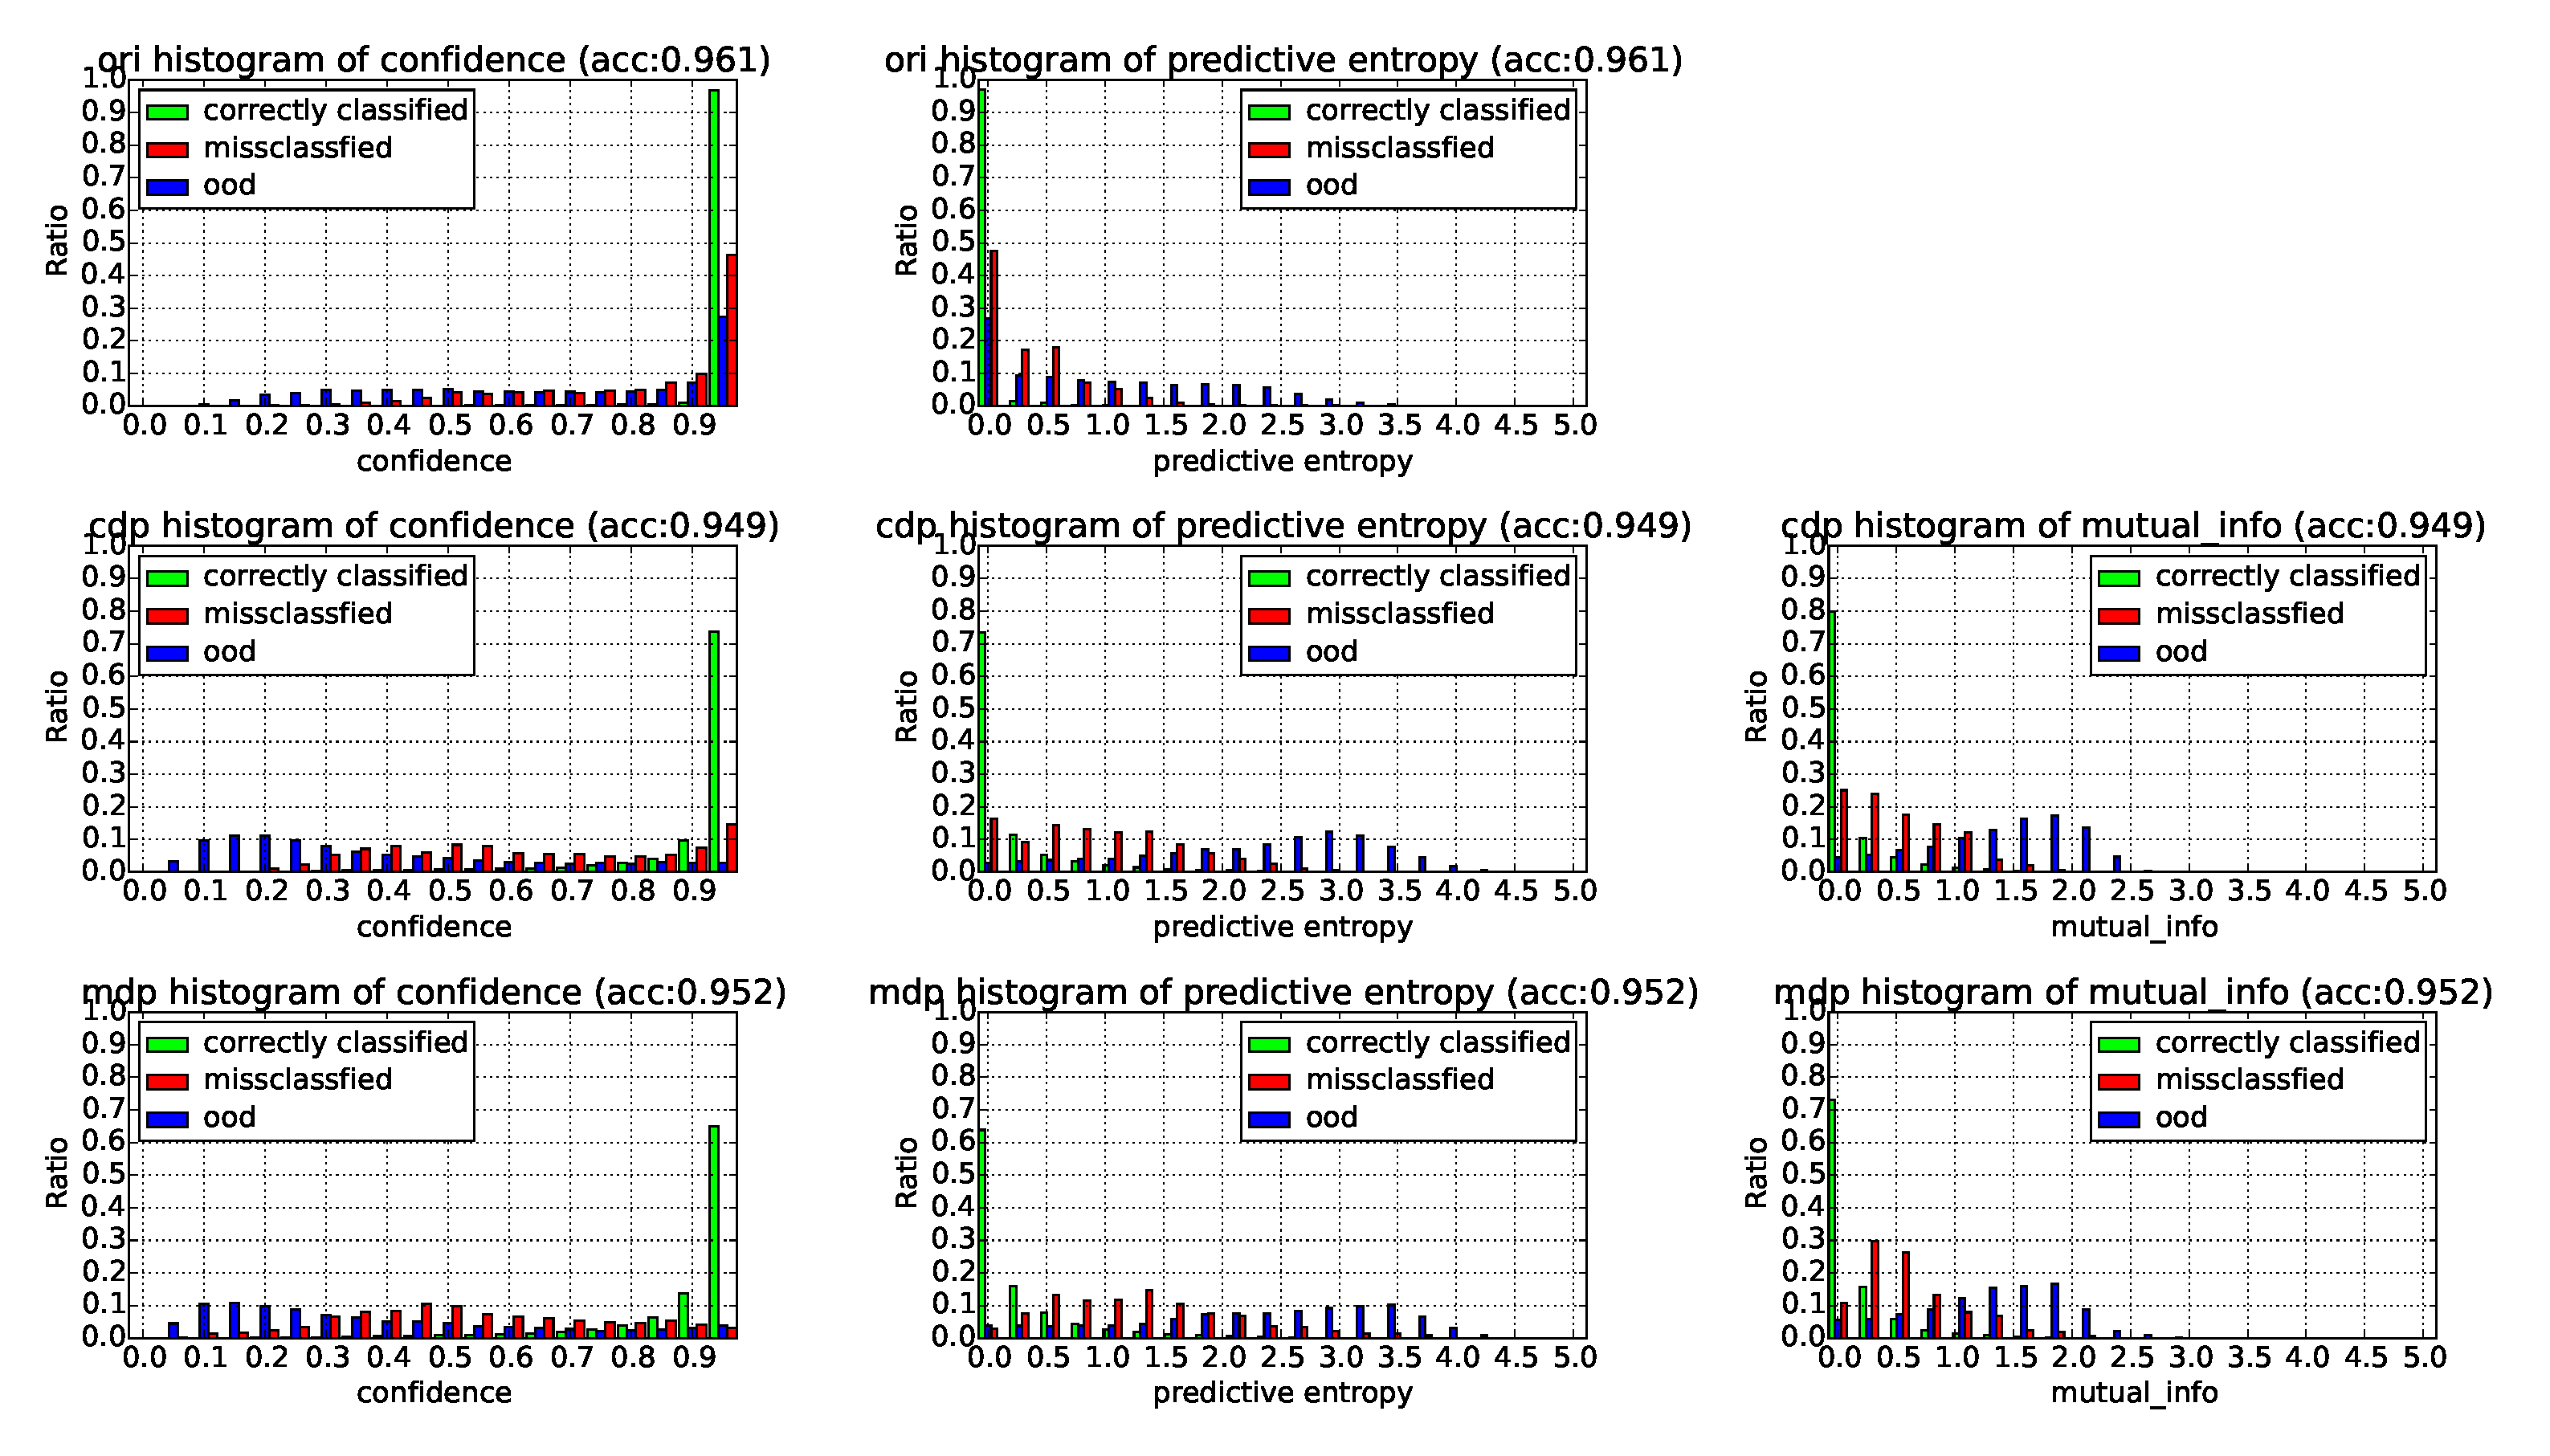
\includegraphics[height=8cm, width=16cm]{uncertainty_estimation/exp1/exp1_histo}
		\caption{Uncertainty(confidence, predictive entropy, mutual information) histograms of original ResNet50, ResNet50 with concrete dropout and ResNet50 with multi-dropout.}		
		\label{exp1_histo}
	\end{center}
\end{figure}
\begin{figure}[H]
	\begin{center}
		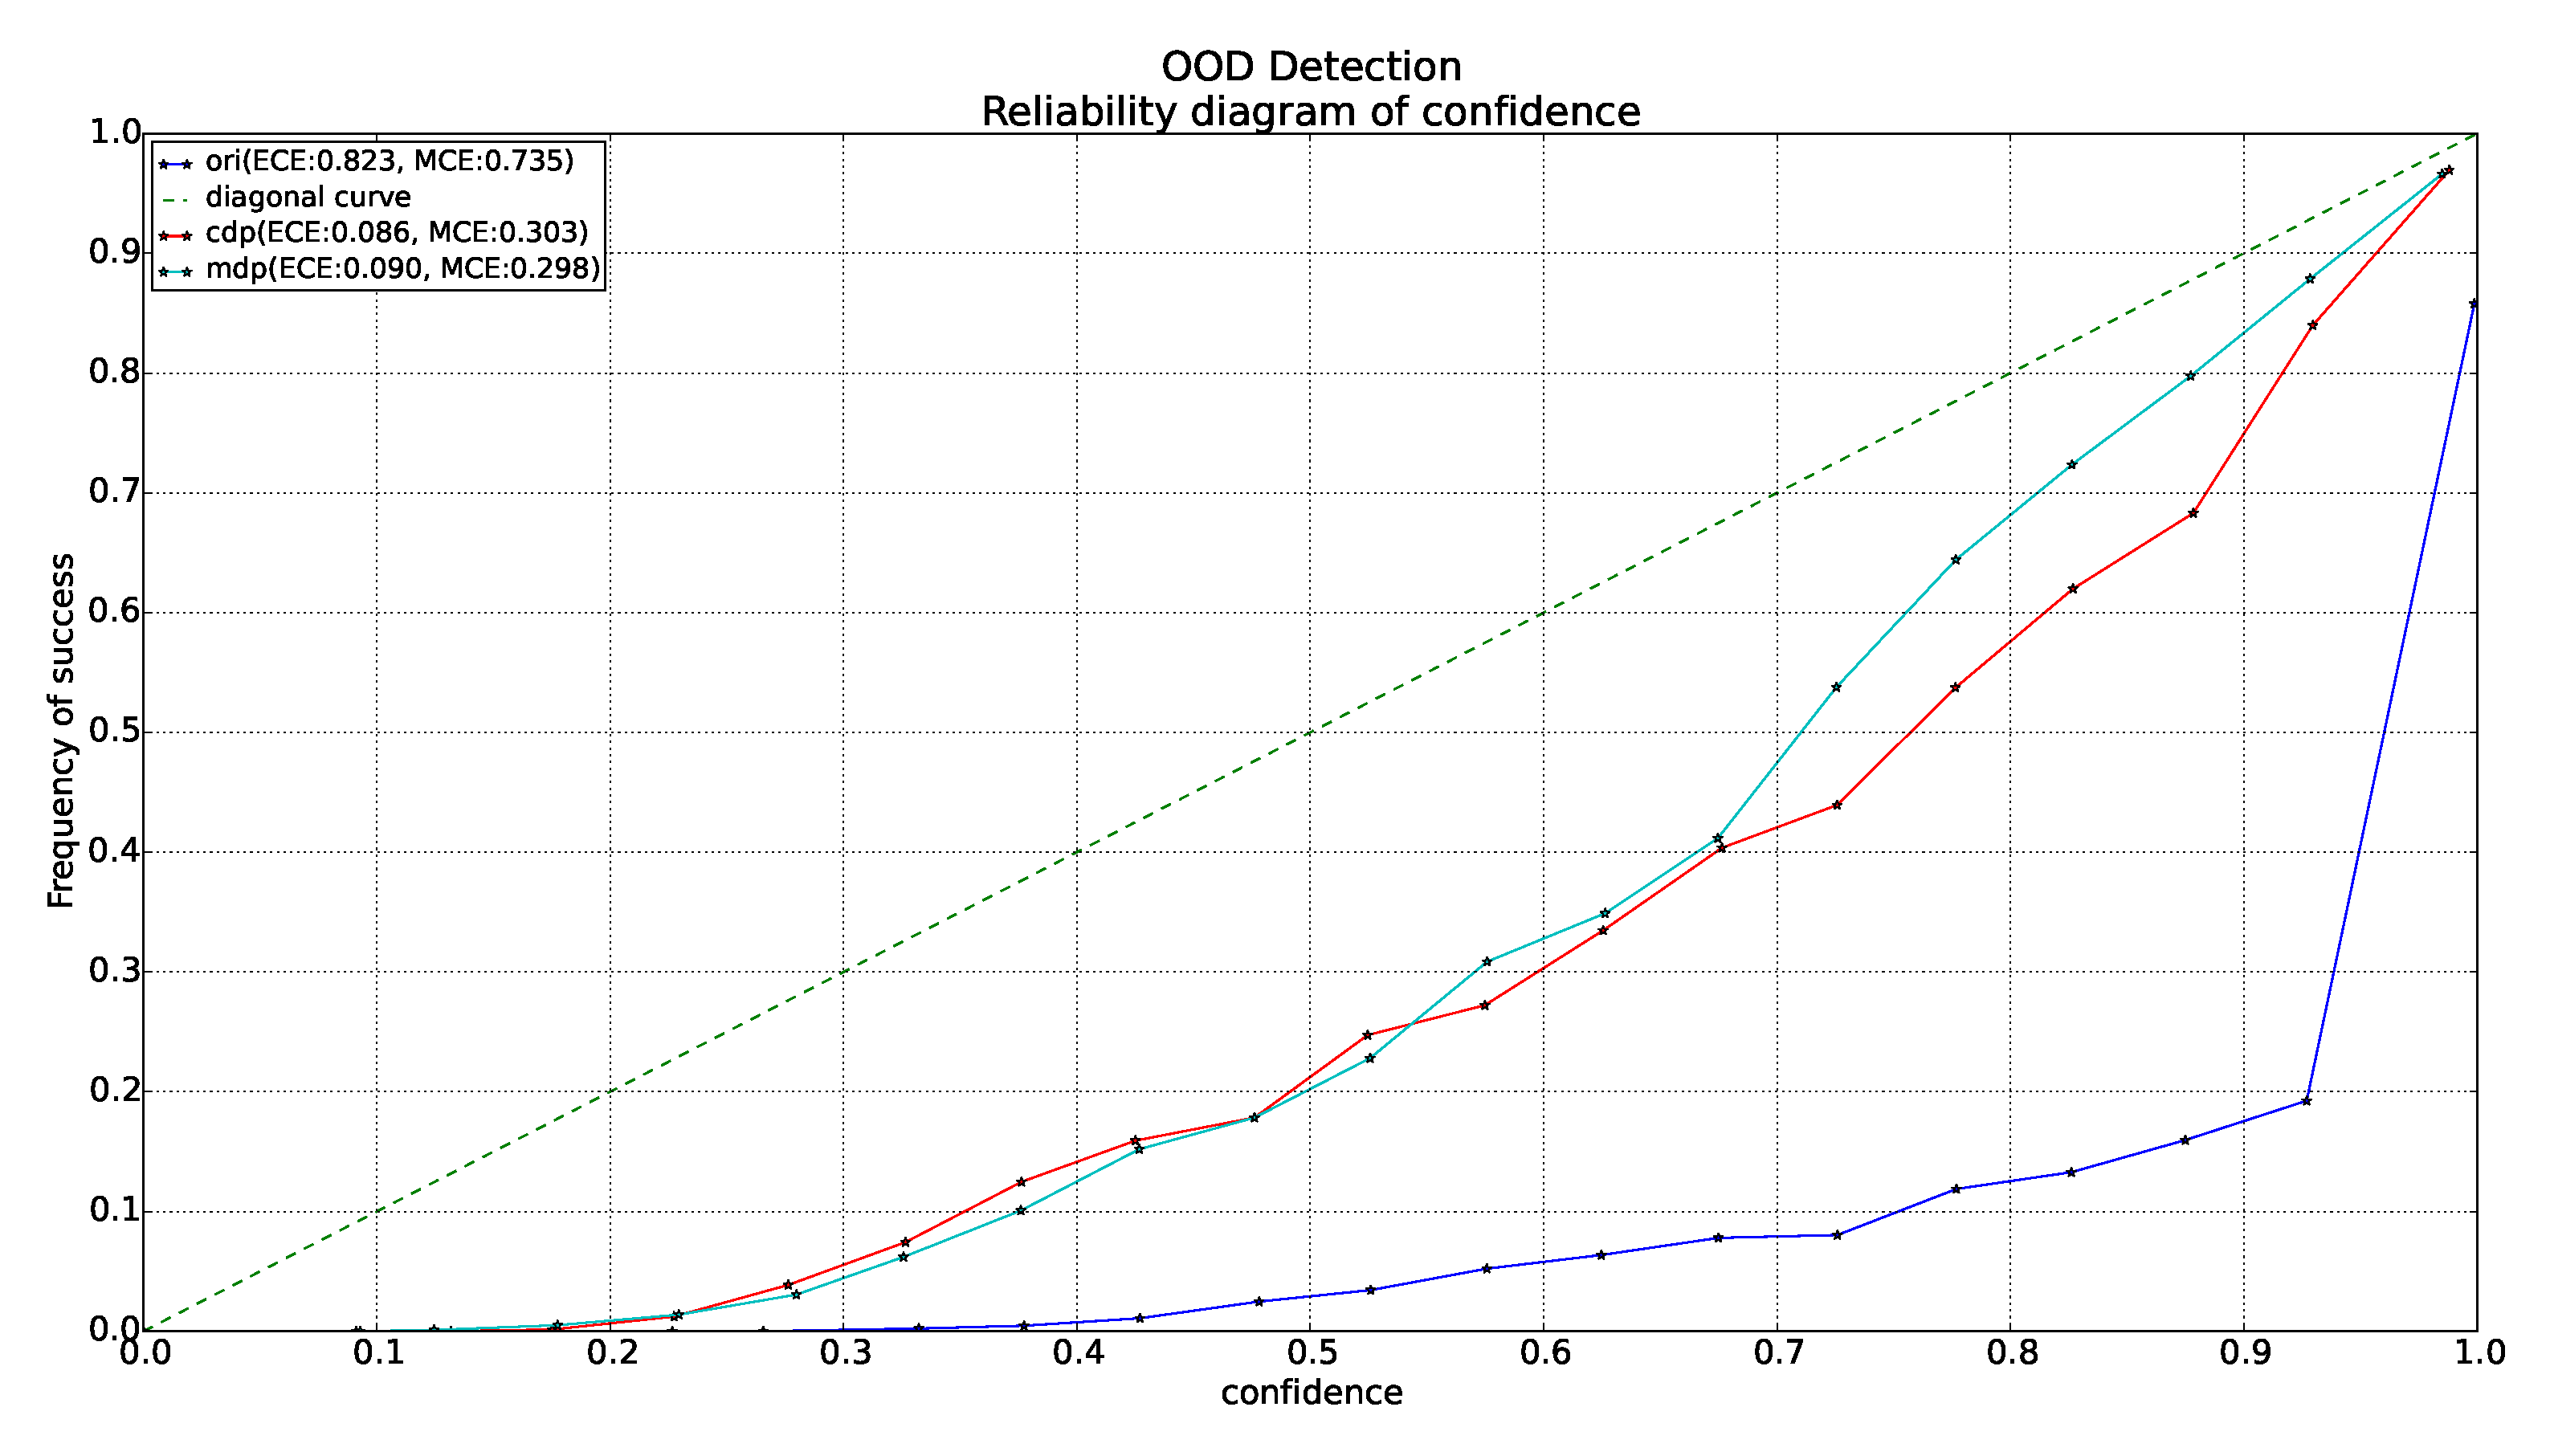
\includegraphics[height=7cm, width=12.5cm]{uncertainty_estimation/exp1/exp1_reliability}
		\caption{Calibration curves of original ResNet50, ResNet50 with concrete dropout and ResNet50 with multi-dropout.}		
		\label{exp1_reliability}
	\end{center}
\end{figure}

\newpage
\subsection{Experiments \RNum{2}}
In this experiment, we evaluate our model on a category recognition task. The difficulties are expressed in two-fold. Firstly, in this task, the model is confronted with classes with more overlapping. Second, because we want to simulate situation of deploying robots in real world scenario and facing data in real world, the UniHB dataset with domain gap(cf. figure\ref{fig:wrgbd2}) to WRGBD is used to achieve this goal. This means, the uncertainty estimation should not only be able to perform well on dataset with exactly same distribution to training set, but also to generalize well to dataset with domain gap which may decrease the accuracy significantly.

Accordingly, we use the entire WRGBD dataset including all view points, whose size is around $160.9\times10^3$, to train our model (in which we split off 20\% of training set as validation set for model selection during training). When it comes to UniHB dataset, we treat objects captured in elevation $30^\circ$ and $60^\circ$ in this dataset as \textbf{adaptation set}, whose size is around $17.1\times10^3$. We test performance of uncertainty estimation on this adaptation dataset. The images of $45^\circ$, whose size is around $8.6\times10^3$ , are used for final evaluation after we fine-tune the model with subset of adaptation set to obtain a domain specific model. The latter part will be experimented in next section. Besides, we also evaluate the uncertainty estimation on OOD dataset(cf. figure \ref{fig:not_in_wrgbd}) whose size is around $6.0\times10^3$. 

There are some protocols for different metrics needed to be clarified, which can help understanding the plots and extracting useful information more easily and quickly.  
\begin{itemize}
	\item The following visual metrics are chosen in one of three runs of different random seeds. The average quantitative results are given in tables following the visual metrics.
	\item The calibration curve with title "Classification" on the left is plotted only on test set. The one with title "OOD detection" on the right is plotted on both OOD dataset and test dataset.
	\item The ROC curve and PR curve measure the separability between two types of prediction.
	The ones with title "classification" on the left measure the separability between \textbf{miss-classification} and \textbf{correct prediction}. The ones with title "OOD detection" on the right measure the separability between \textbf{OOD prediction} and \textbf{correct prediction}.
	\item As is shown in uncertainty histogram, we have used three uncertainty measures. Each one has its own ROC curve and PR curve of correct prediction versus miss-classification or OOD prediction. In the following results of ROC curve and PR curve, we only show the one with highest area under curve. In detail, \textbf{Confidence} is chosen in case of correct prediction versus miss-classification. \textbf{Mutual information} is chosen in case of correct prediction versus OOD prediction.
\end{itemize}   

\subsection{Comparison with Ensemble}

\paragraph{Uncertainty histogram}
This is uncertainty hitsogram
\begin{figure}[H]
	\begin{center}
		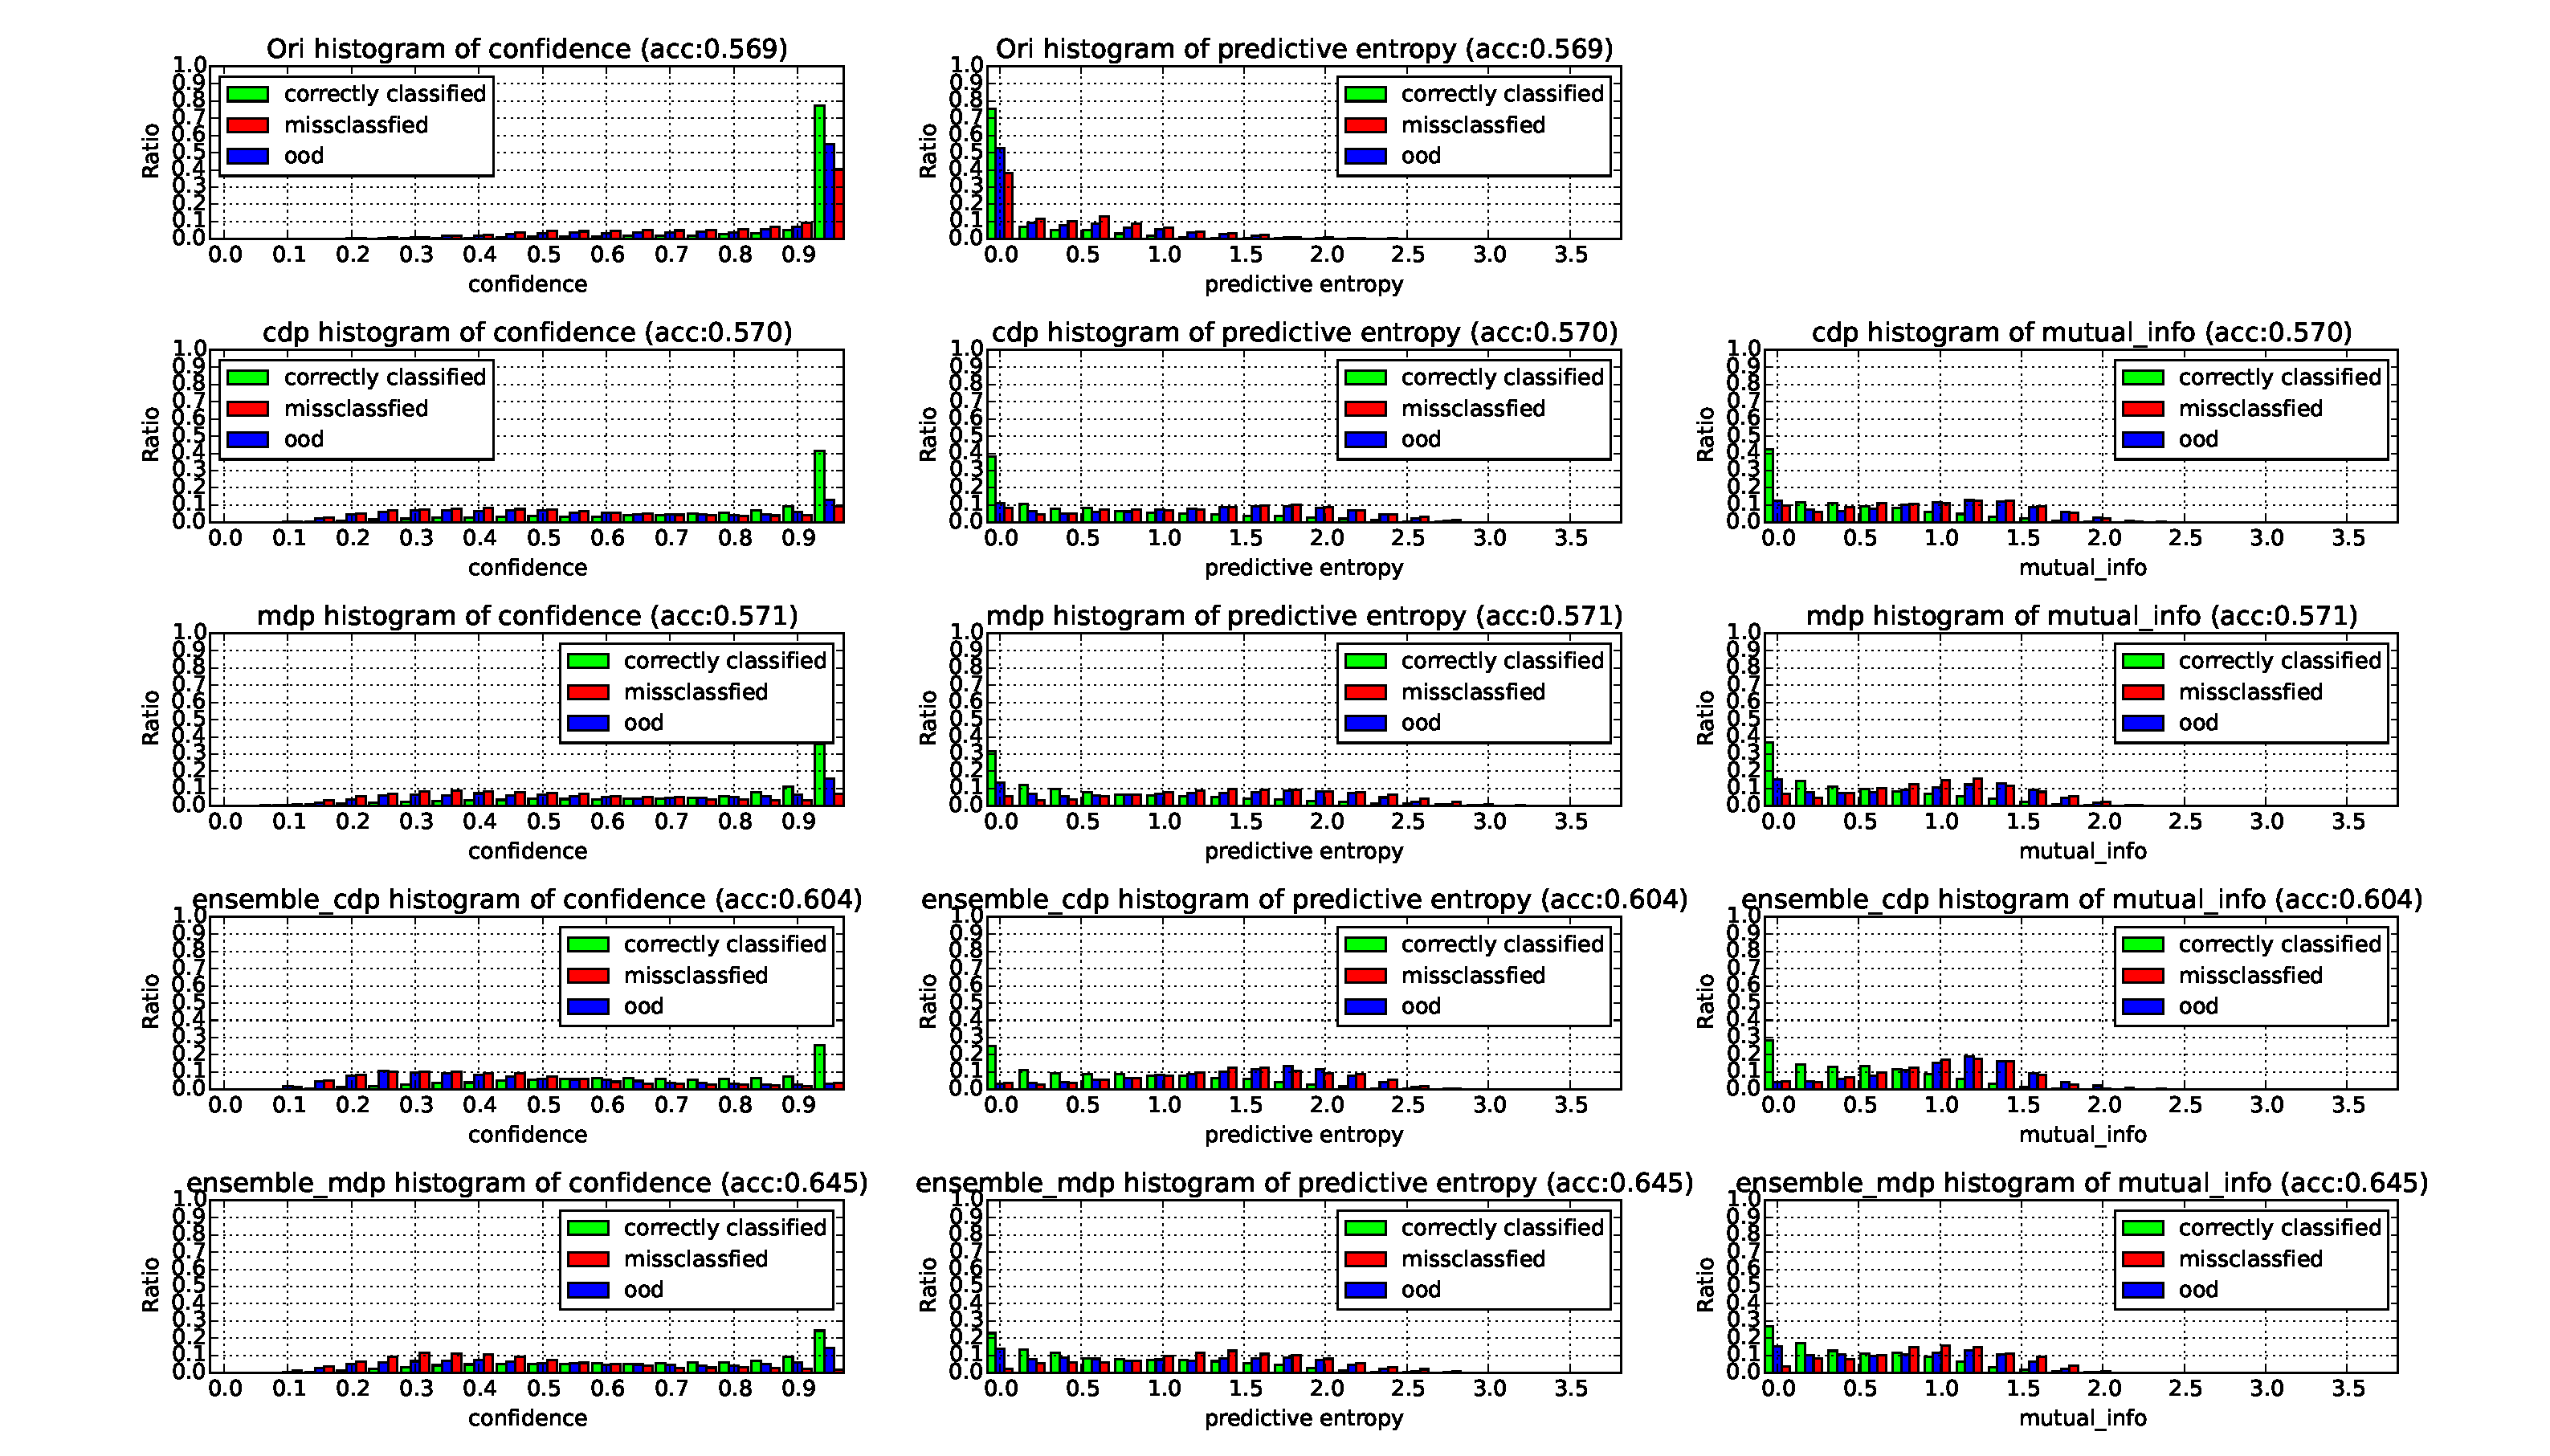
\includegraphics[height=13cm, width=16cm]{uncertainty_estimation/hist_seed3_ensemble}
		\caption{Uncertainty histogram of one of three runs.}		
		\label{exp1_reliability}
	\end{center}
\end{figure}
\paragraph{Reliability diagram}
This is Reliability diagram
\begin{figure}[H]
	\begin{center}
		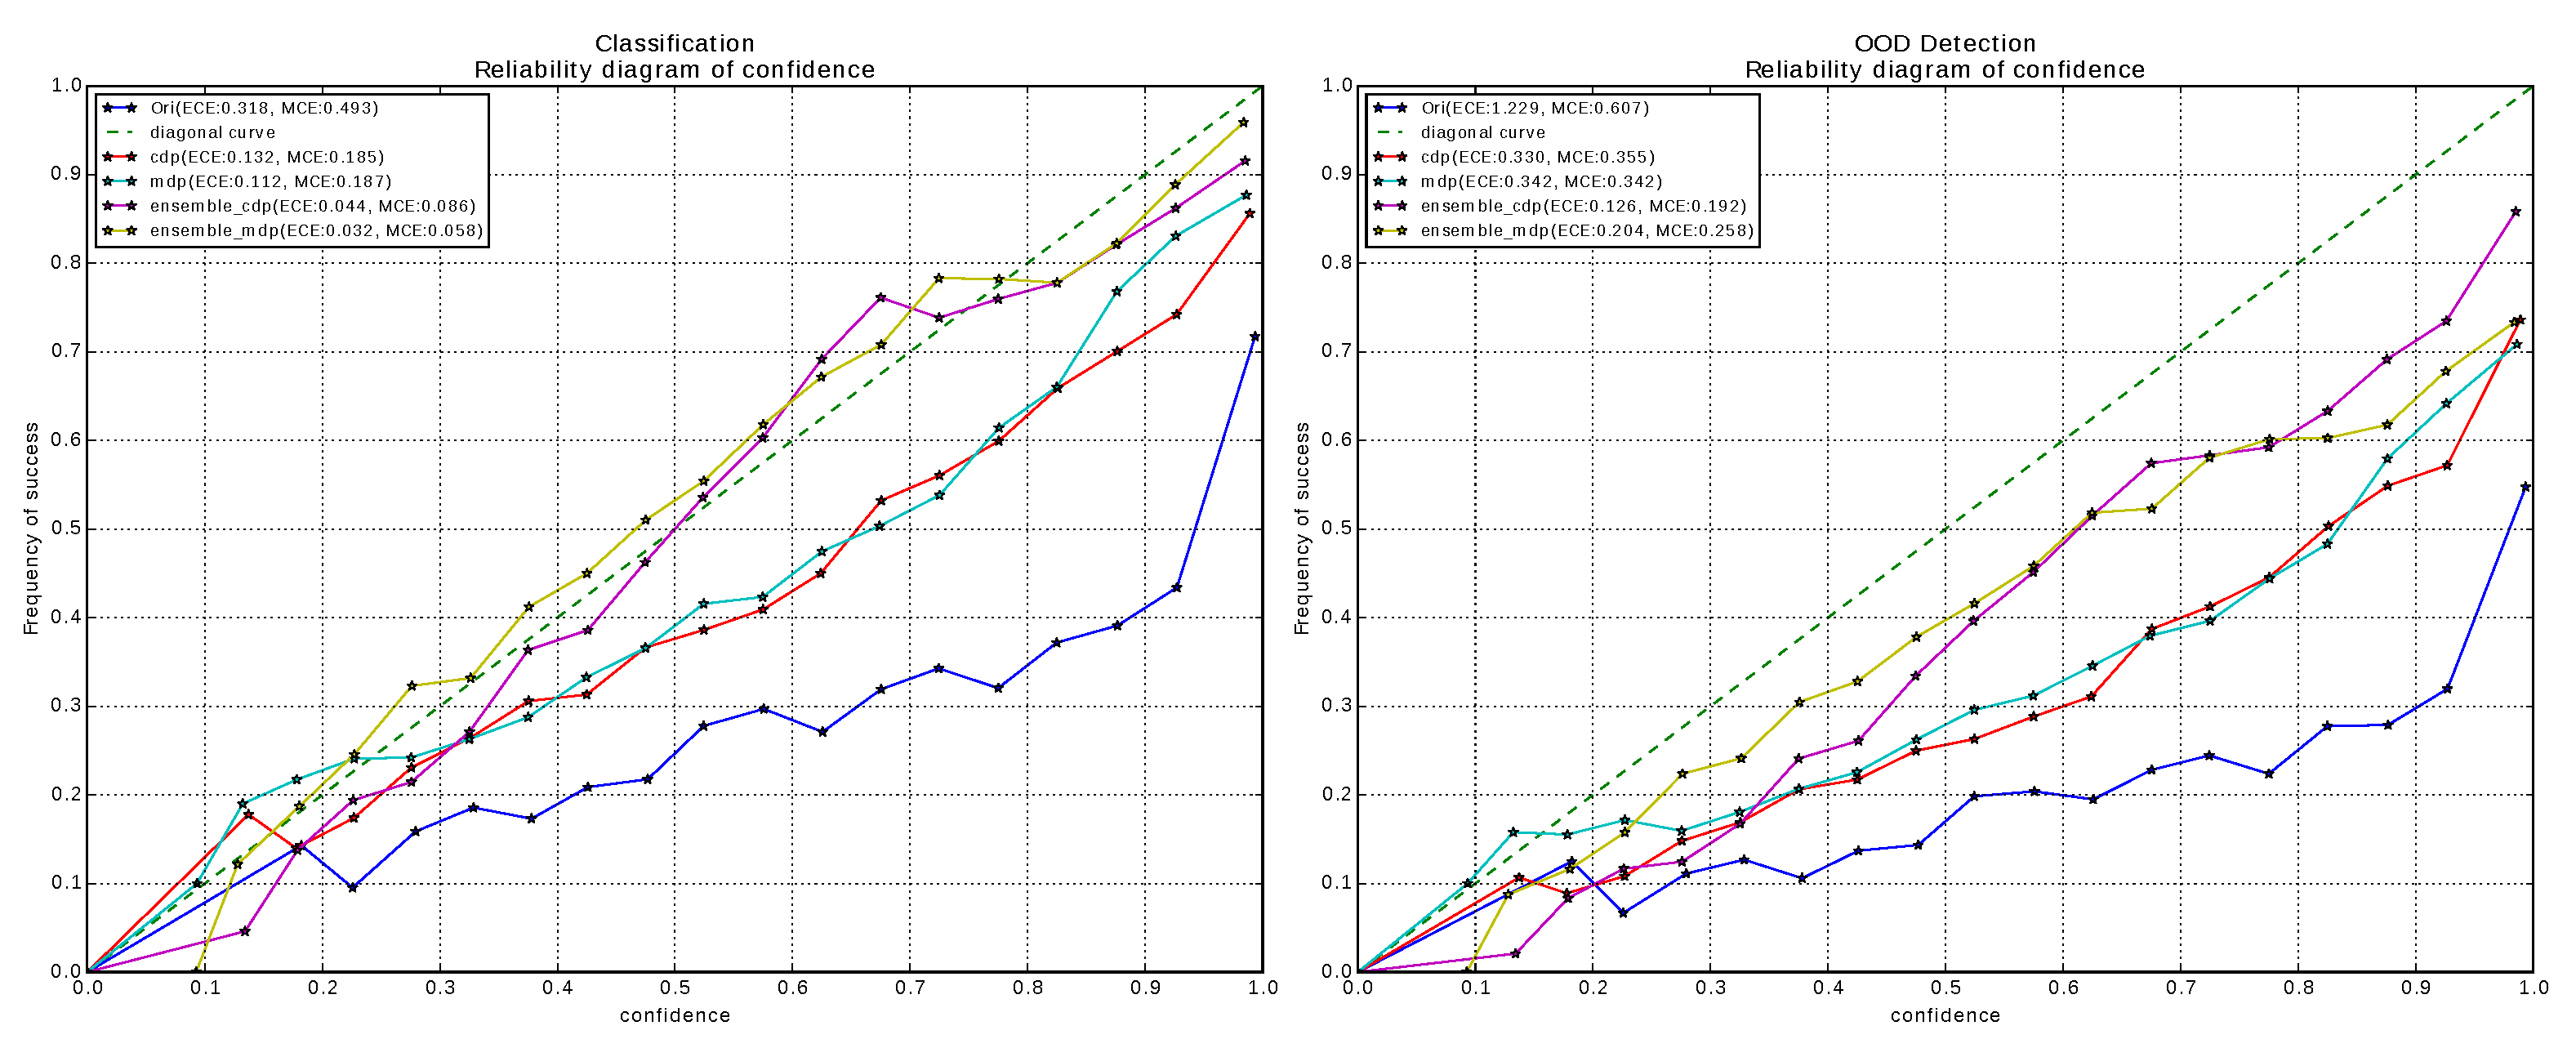
\includegraphics[height=6cm, width=16.5cm]{uncertainty_estimation/reliability_seed3_ensemble_}
		\caption{Calibration curve of one of three runs.}		
		\label{exp1_reliability}
	\end{center}
\end{figure}

\paragraph{ROC curve and PR curve}
This is ROC and PR curve
\begin{figure}[H]
	\begin{center}
		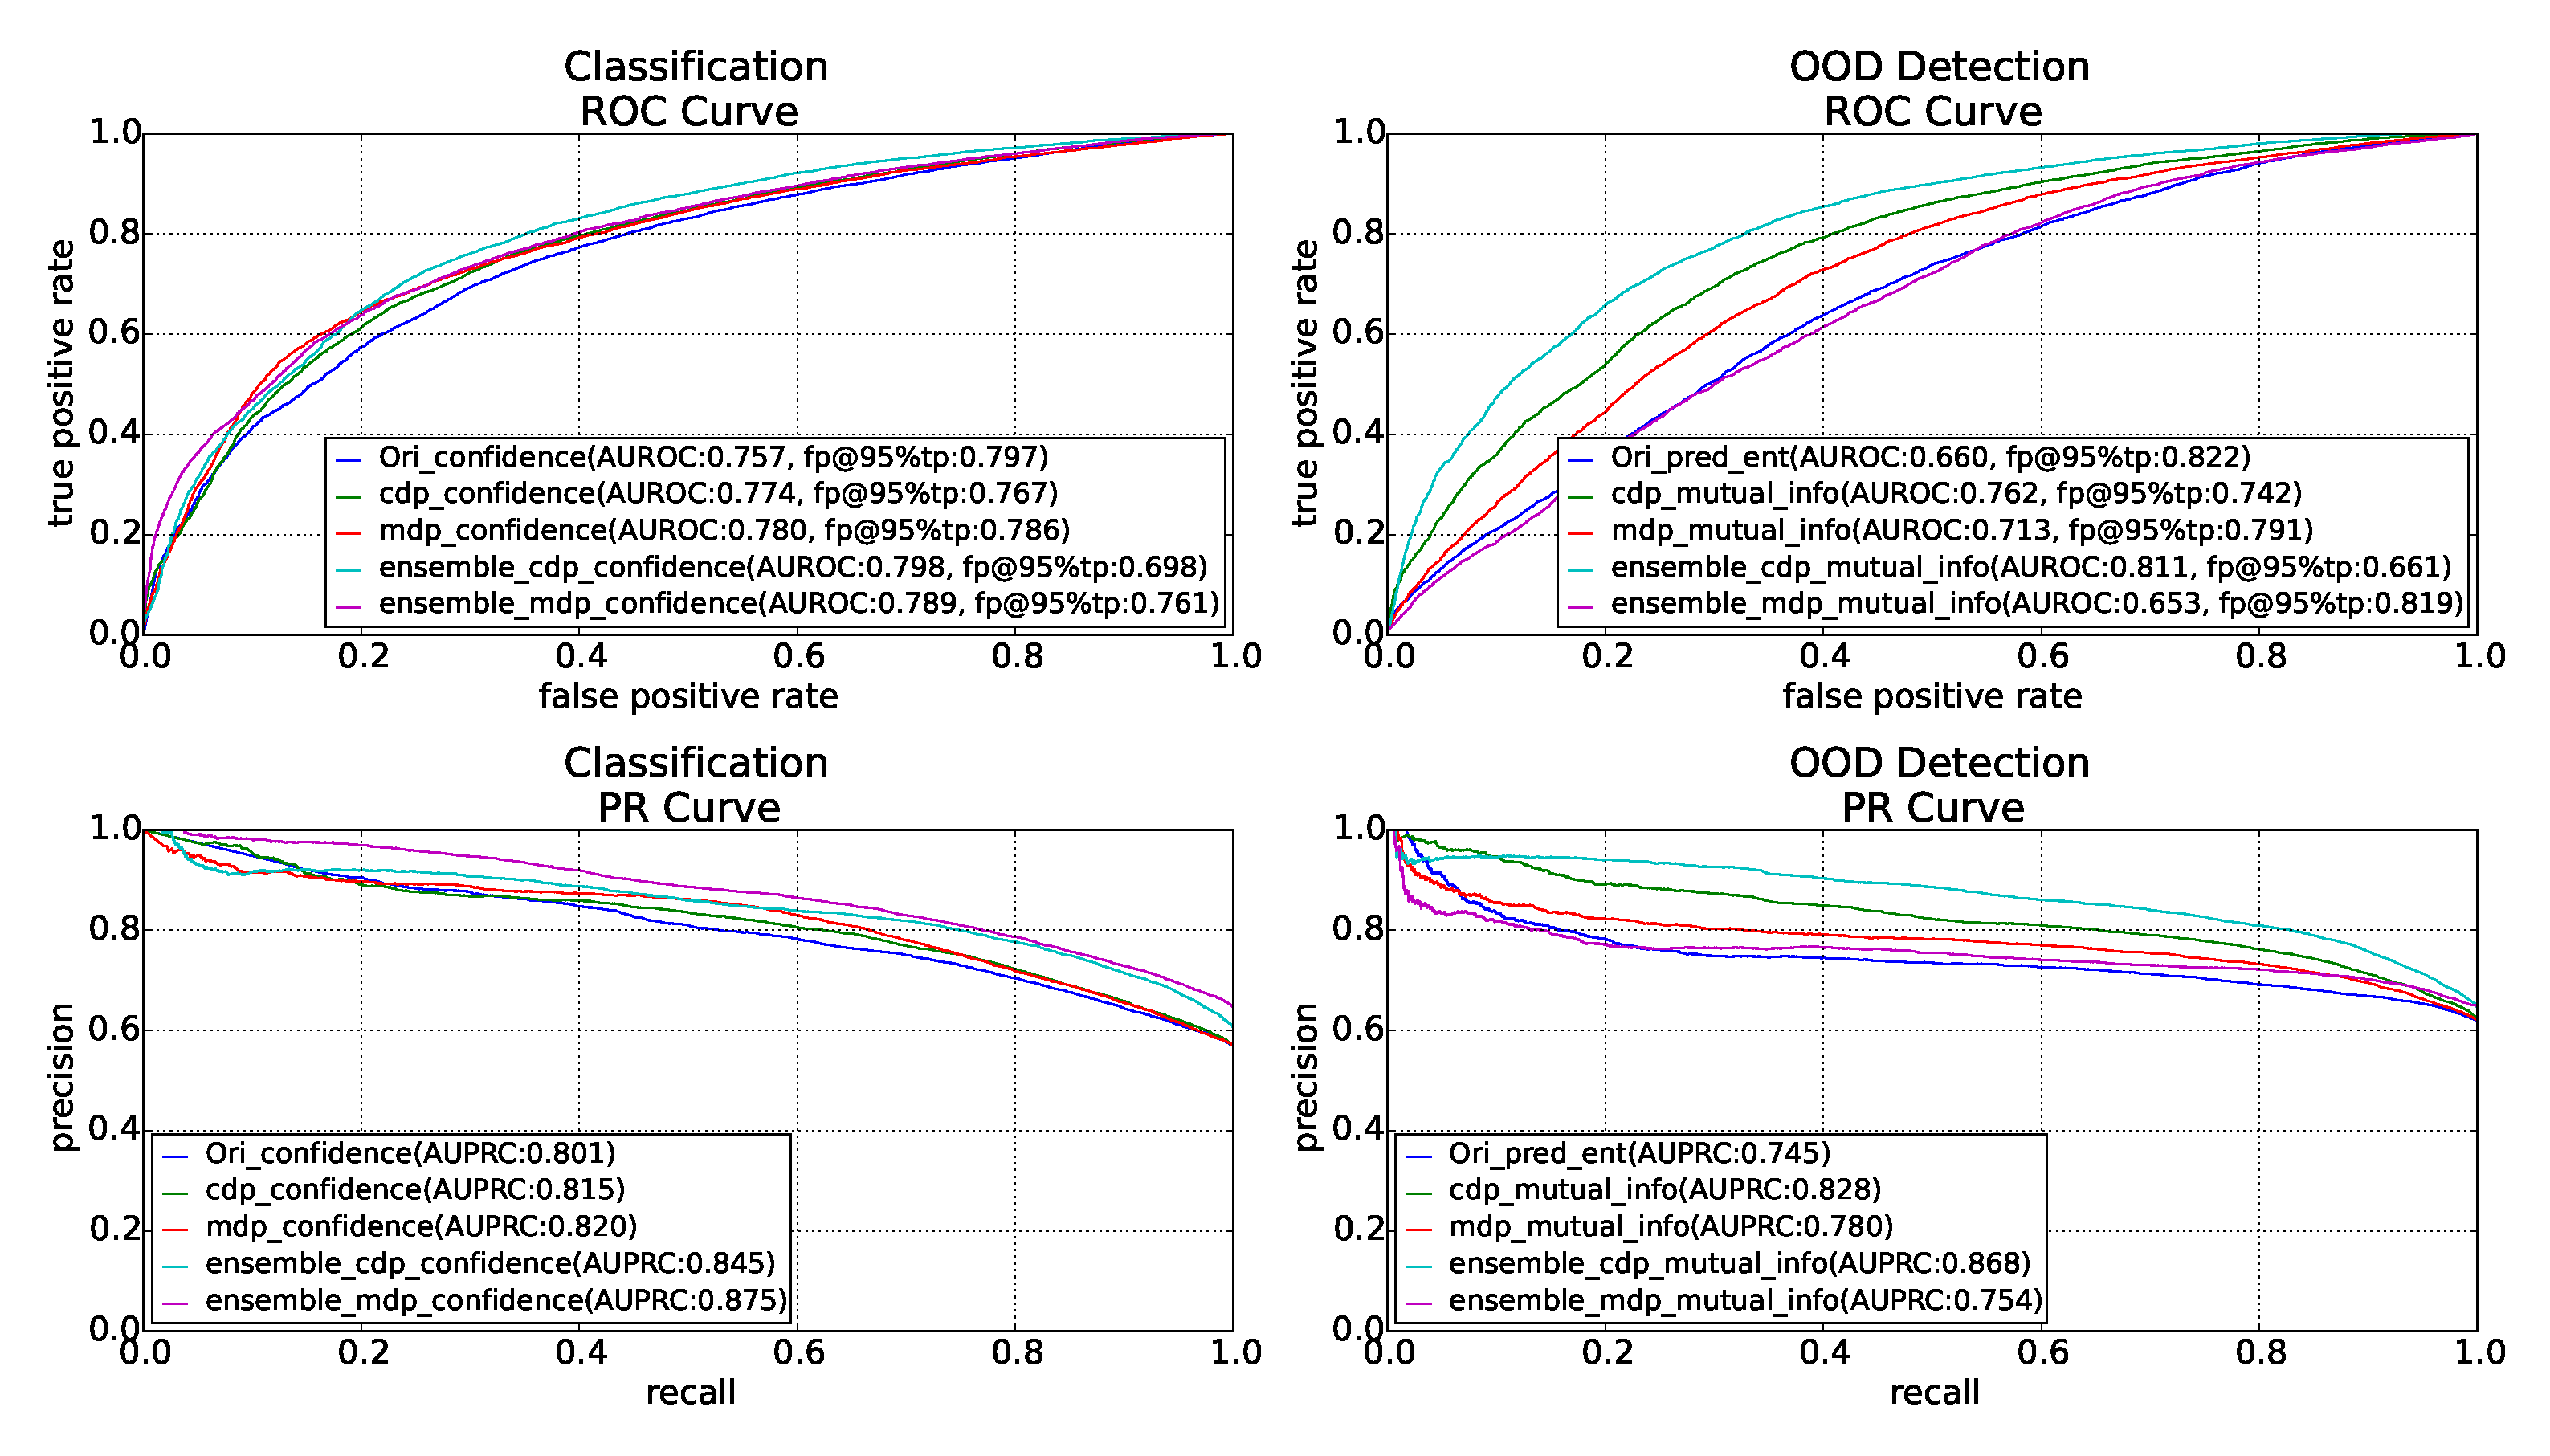
\includegraphics[height=9cm, width=16cm]{uncertainty_estimation/roc_pr_seed3_ensemble}
		\caption{ROC and PR curve of one of three runs.}		
		\label{exp1_reliability}
	\end{center}
\end{figure}

\begin{table}[H]
	\centering
	\caption{results of acc, bs, nll, ece, mce, auroc, aupr}
	\begin{tabular}{|l|l|l|l|}
		\hline
		& accuracy$ \boldsymbol\uparrow$     & brier\_score $ \boldsymbol \downarrow$& \begin{tabular}[c]{@{}l@{}}negative\\ log \\ likelihood $ \boldsymbol\downarrow$\end{tabular} \\ \hline
		ori           & 0.568$\pm$0.008 & 0.722$\pm$0.019 & 3.242$\pm$0.340                                                         \\ \hline
		cdp           & 0.577$\pm$0.008 & 0.594$\pm$0.013 & 2.088$\pm$0.181                                                         \\ \hline
		mdp           & 0.599$\pm$0.023 & 0.566$\pm$0.020 & 1.940$\pm$0.064                                                         \\ \hline
		emsemble\_cdp & 0.604        & 0.534        & 1.452                                                                \\ \hline
		emsemble\_mdp & 0.645        & 0.496        & 1.389                                                                \\ \hline
	\end{tabular}
\label{table:compareWithEnsemble}
\end{table}

\begin{table}[H]
	\centering
	% \caption{results of ece, mce, auroc, aupr}
	\begin{tabular}{|l|l|l|l|l|}
		\hline
		& \begin{tabular}[c]{@{}l@{}}expected\\ calibration\\ error(w/o. OOD/\\ w. OOD)$ \boldsymbol\downarrow$\end{tabular} & \begin{tabular}[c]{@{}l@{}}maximal\\ calibration\\ error(w/o. OOD/\\ w. OOD)$ \boldsymbol\downarrow$\end{tabular} & \begin{tabular}[c]{@{}l@{}}area under\\ ROC\\ (vs. Miss-\\ classified/\\ vs. OOD)$ \boldsymbol\uparrow$\end{tabular} & \begin{tabular}[c]{@{}l@{}}area under\\ PR curve\\ (vs. Miss-\\ classified/\\ vs. OOD)$ \boldsymbol\uparrow$\end{tabular} \\ \hline
		ori           & \begin{tabular}[c]{@{}l@{}}0.304$\pm$0.016 /\\ 0.633$\pm$0.065\end{tabular}                      & \begin{tabular}[c]{@{}l@{}}0.461$\pm$0.027 /\\ 0.362$\pm$0.025\end{tabular}                     & \begin{tabular}[c]{@{}l@{}}0.750$\pm$0.007 /\\ 0.664$\pm$0.011\end{tabular}           & \begin{tabular}[c]{@{}l@{}}0.802$\pm$0.008 /\\ 0.751$\pm$0.018\end{tabular}                \\ \hline
		cdp           & \begin{tabular}[c]{@{}l@{}}0.124$\pm$0.023/\\ 0.288$\pm$0.048\end{tabular}                         & \begin{tabular}[c]{@{}l@{}}0.206$\pm$0.015/ \\ 0.374$\pm$0.018\end{tabular}                     & \begin{tabular}[c]{@{}l@{}}0.775$\pm$0.008/ \\ 0.783$\pm$0.022\end{tabular}           & \begin{tabular}[c]{@{}l@{}}0.825$\pm$0.007/ \\ 0.850$\pm$0.022\end{tabular}                \\ \hline
		mdp           & \begin{tabular}[c]{@{}l@{}}0.114$\pm$0.012/ \\ 0.383$\pm$0.046\end{tabular}                      & \begin{tabular}[c]{@{}l@{}}0.199$\pm$0.016/ \\ 0.367$\pm$0.023\end{tabular}                     & \begin{tabular}[c]{@{}l@{}}0.780$\pm$0.011/ \\ 0.709$\pm$0.004\end{tabular}           & \begin{tabular}[c]{@{}l@{}}0.838$\pm$0.013/ \\ 0.788$\pm$0.006\end{tabular}                \\ \hline
		emsemble\_cdp & \begin{tabular}[c]{@{}l@{}}0.044/\\0.042 \end{tabular} 
		 &  \begin{tabular}[c]{@{}l@{}}0.086/\\0.093 \end{tabular}                                                                                    & \begin{tabular}[c]{@{}l@{}}0.798/\\0.811  \end{tabular}                                                                           & \begin{tabular}[c]{@{}l@{}}0.845/\\0.868  \end{tabular}                                                                                \\ \hline
		emsemble\_mdp & \begin{tabular}[c]{@{}l@{}}0.032/\\0.170 \end{tabular}                                                                                       & \begin{tabular}[c]{@{}l@{}}0.058/\\0.227  \end{tabular}                                                                                     & \begin{tabular}[c]{@{}l@{}}0.789/\\0.653 \end{tabular}                                                                            & \begin{tabular}[c]{@{}l@{}}0.875/\\0.754  \end{tabular}                                                                                \\ \hline
	\end{tabular}
\end{table}	


\subsection{Comparison with Laplace approximation}
Because Laplace approximation requires only MAP point estimate of parameter, re-training the model is not needed. Therefore we take the already trained model of different approaches as our MAP point estimate. We set the scale parameter of kronecker factors as $1$ and dump factor as $15$ based on grid search on the validation set.   
his is uncertainty hitsogram
\begin{figure}[H]
	\begin{center}
		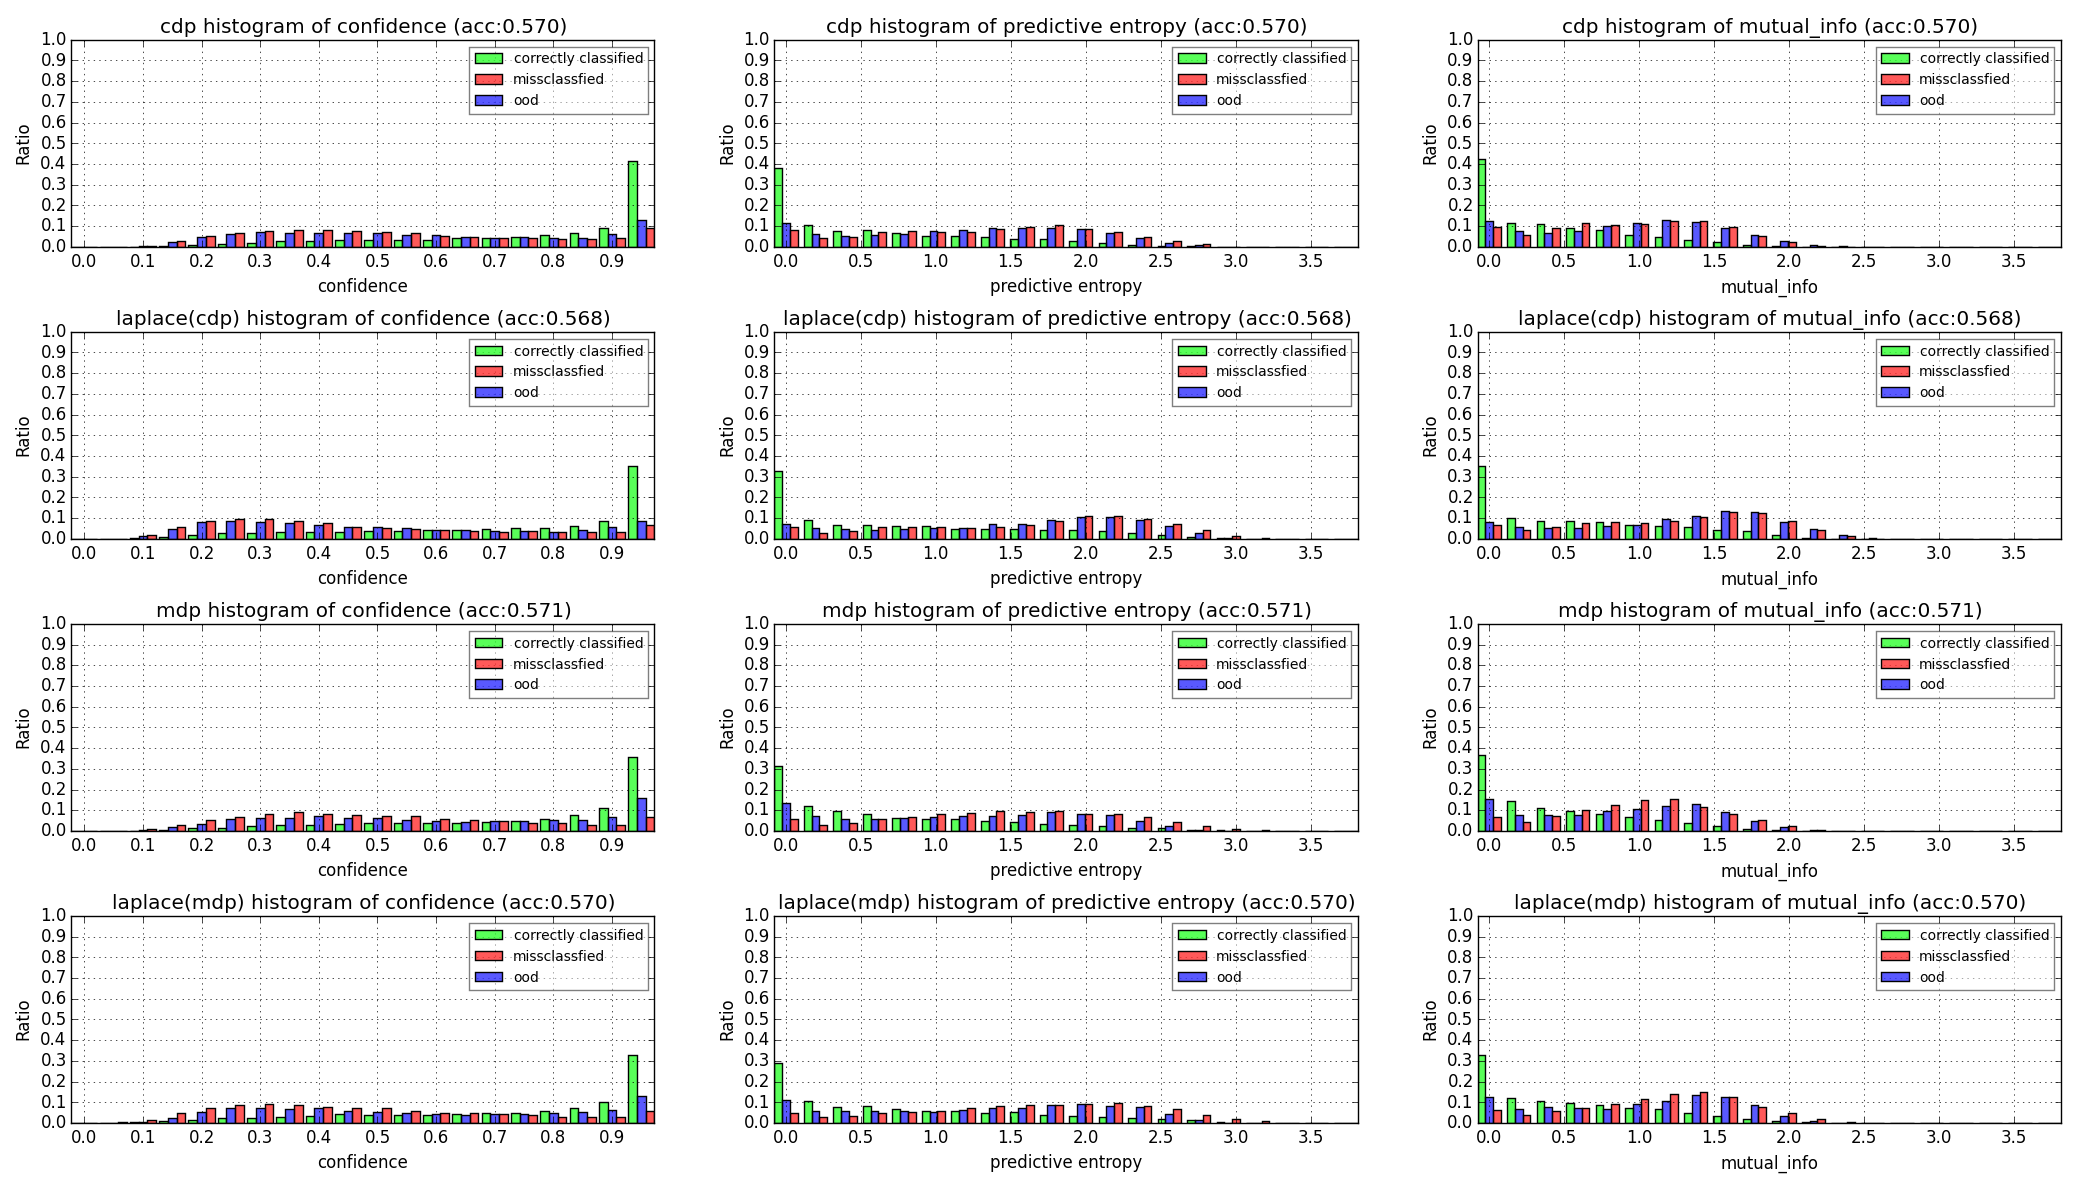
\includegraphics[height=11cm, width=16cm]{uncertainty_estimation/laplace/histo_ood_seed3}
		\caption{Uncertainty histogram of one of three runs.}		
		\label{exp1_reliability}
	\end{center}
\end{figure}

This is Reliability diagram
\begin{figure}[H]
	\begin{center}
		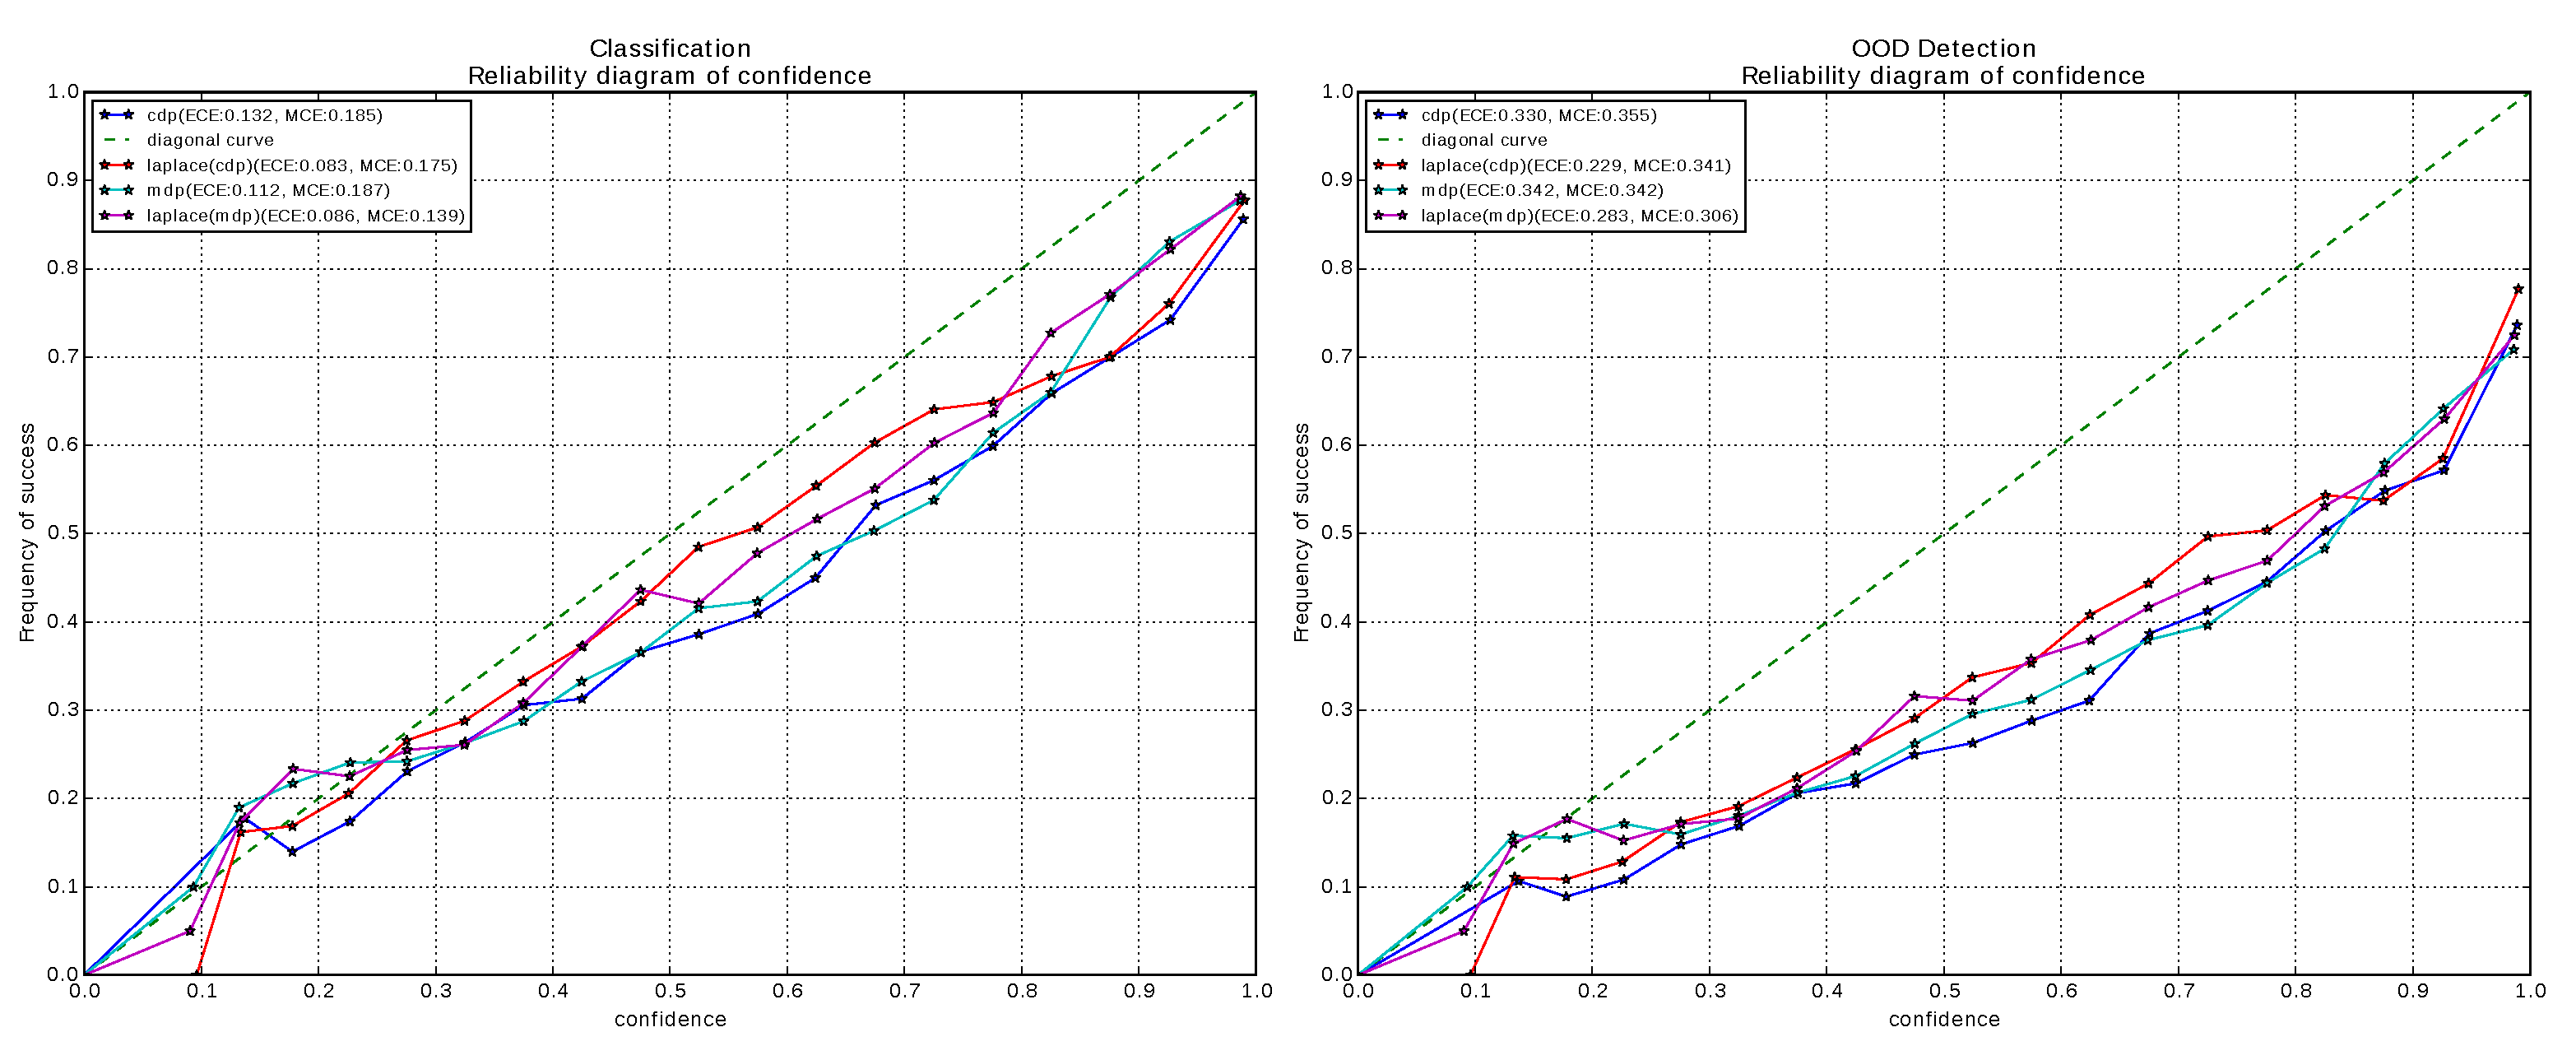
\includegraphics[height=5cm, width=16.5cm]{uncertainty_estimation/laplace/reliabilty_seed3_}
		\caption{Calibration curve of one of three runs.}		
		\label{exp1_reliability}
	\end{center}
\end{figure}

This is ROC and PR curve
\begin{figure}[H]
	\begin{center}
		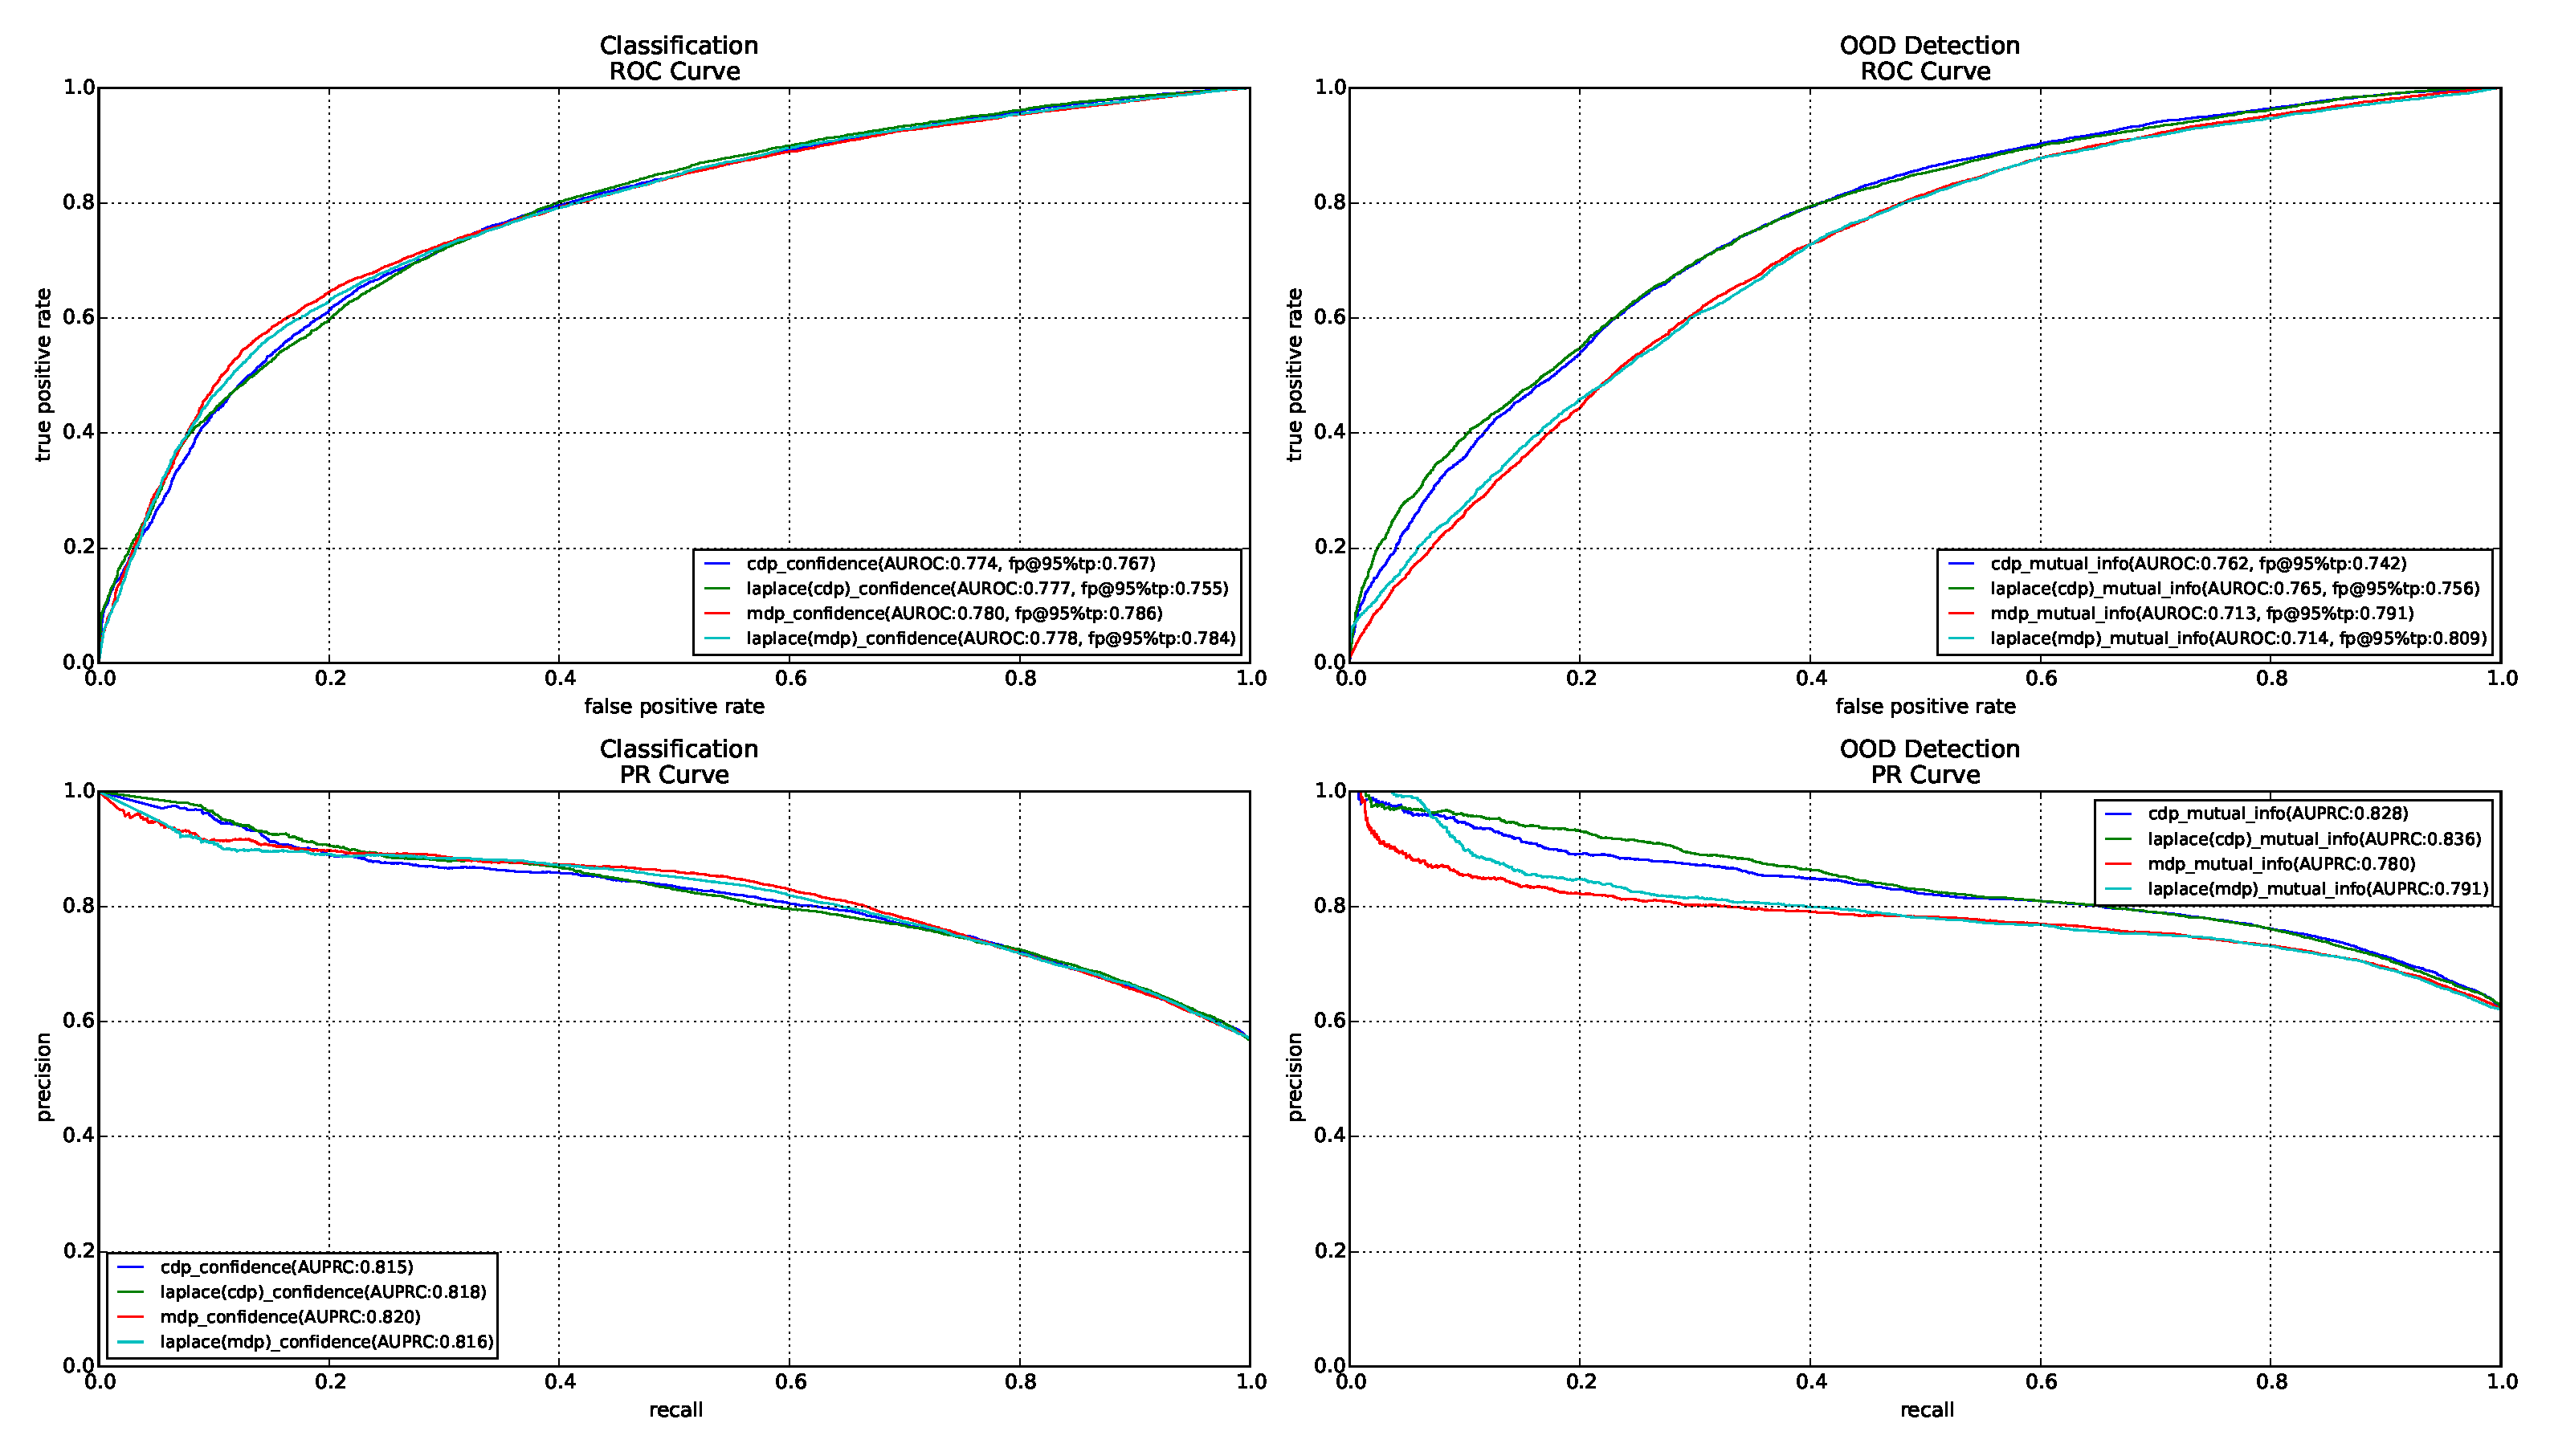
\includegraphics[height=9cm, width=16cm]{uncertainty_estimation/laplace/roc_pr_seed3}
		\caption{ROC and PR curve of one of three runs.}		
		\label{exp1_reliability}
	\end{center}
\end{figure}

\begin{table}[H]
	\centering
	\begin{tabular}{|l|l|l|l|}
		\hline
		& accuracy  $\boldsymbol \uparrow$                                                            & brier score $\boldsymbol \downarrow$                                                           & \begin{tabular}[c]{@{}l@{}}negative \\ log\\ likelihood $\boldsymbol \downarrow$\end{tabular}  \\ \hline
		cdp          & 
		\begin{tabular}[c]{@{}l@{}}0.577$\pm$0.008\end{tabular} & 
		\begin{tabular}[c]{@{}l@{}}0.594$\pm$0.013\end{tabular} & \begin{tabular}[c]{@{}l@{}}2.088$\pm$0.181\end{tabular} \\ \hline
		
		laplace\_cdp & 
		\begin{tabular}[c]{@{}l@{}}0.576$\pm$0.009\end{tabular}    & \begin{tabular}[c]{@{}l@{}}0.602$\pm$0.011\end{tabular} & \begin{tabular}[c]{@{}l@{}}2.322$\pm$0.350\end{tabular} \\ \hline
		
		mdp          & 
		\begin{tabular}[c]{@{}l@{}}0.599$\pm$0.023\end{tabular} & \begin{tabular}[c]{@{}l@{}}0.566$\pm$0.020\end{tabular} & \begin{tabular}[c]{@{}l@{}}1.940$\pm$0.064\end{tabular} \\ \hline
		laplace\_mdp & 		\begin{tabular}[c]{@{}l@{}}0.598$\pm$0.024\end{tabular} & \begin{tabular}[c]{@{}l@{}}0.567$\pm$0.018\end{tabular} & \begin{tabular}[c]{@{}l@{}}1.970$\pm$0.117\end{tabular} \\ \hline
	\end{tabular}
\end{table}
\begin{table}[H]
	\centering
	\begin{tabular}{|l|l|l|l|l|}
		\hline
		& \begin{tabular}[c]{@{}l@{}}expected\\ calibration\\ error(w/o. OOD/\\ w. OOD) $\boldsymbol \downarrow$\end{tabular} & \begin{tabular}[c]{@{}l@{}}maximal\\ calibration\\ error(w/o. OOD/\\ w. OOD)$\boldsymbol \downarrow$\end{tabular} & \begin{tabular}[c]{@{}l@{}}area under\\ ROC\\ (vs. Miss-\\ classified/\\ vs. OOD)$\boldsymbol \uparrow$\end{tabular} & \begin{tabular}[c]{@{}l@{}}area under\\ PR curve\\ (vs. Miss-\\ classified/\\ vs. OOD)$\boldsymbol \uparrow$\end{tabular} \\ \hline
		
		cdp          & \begin{tabular}[c]{@{}l@{}}0.124$\pm$0.023/ \\0.288$\pm$0.048\end{tabular}                      & \begin{tabular}[c]{@{}l@{}}0.206$\pm$0.015/ \\0.374$\pm$0.018\end{tabular}                     & \begin{tabular}[c]{@{}l@{}}0.775$\pm$0.008/ \\0.783$\pm$0.022\end{tabular}           & \begin{tabular}[c]{@{}l@{}}0.825$\pm$0.007/ \\0.850$\pm$0.022\end{tabular}                \\ \hline
		
		laplace\_cdp & \begin{tabular}[c]{@{}l@{}}0.129$\pm$0.058/ \\0.341$\pm$0.157\end{tabular}                         & \begin{tabular}[c]{@{}l@{}}0.235$\pm$0.073/ \\0.406$\pm$0.070\end{tabular}                     & \begin{tabular}[c]{@{}l@{}}0.779$\pm$0.004/ \\0.782$\pm$0.017\end{tabular}           & \begin{tabular}[c]{@{}l@{}}0.826$\pm$0.007/ \\0.849$\pm$0.016\end{tabular}                \\ \hline
		
		mdp          & \begin{tabular}[c]{@{}l@{}}0.114$\pm$0.012/ \\0.383$\pm$0.046\end{tabular}                      & \begin{tabular}[c]{@{}l@{}}0.199$\pm$0.016/ \\0.367$\pm$0.023\end{tabular}                     & \begin{tabular}[c]{@{}l@{}}0.780$\pm$0.011/ \\0.709$\pm$0.004\end{tabular}           & \begin{tabular}[c]{@{}l@{}}0.838$\pm$0.013/ \\0.788$\pm$0.006\end{tabular}                \\ \hline
		
		laplace\_mdp         & \begin{tabular}[c]{@{}l@{}} 0.104$\pm$0.018/ \\0.352$\pm$0.061\end{tabular}                      & \begin{tabular}[c]{@{}l@{}}0.179$\pm$0.029/ \\0.352$\pm$0.038\end{tabular}                     & \begin{tabular}[c]{@{}l@{}}0.776$\pm$0.012/ \\0.711$\pm$0.005\end{tabular}           & \begin{tabular}[c]{@{}l@{}}0.837$\pm$0.015/ \\0.798$\pm$0.005\end{tabular}                \\ \hline
	\end{tabular}
\end{table}
\subsection{Ablation study}

\begin{figure}[H]
	\begin{center}
		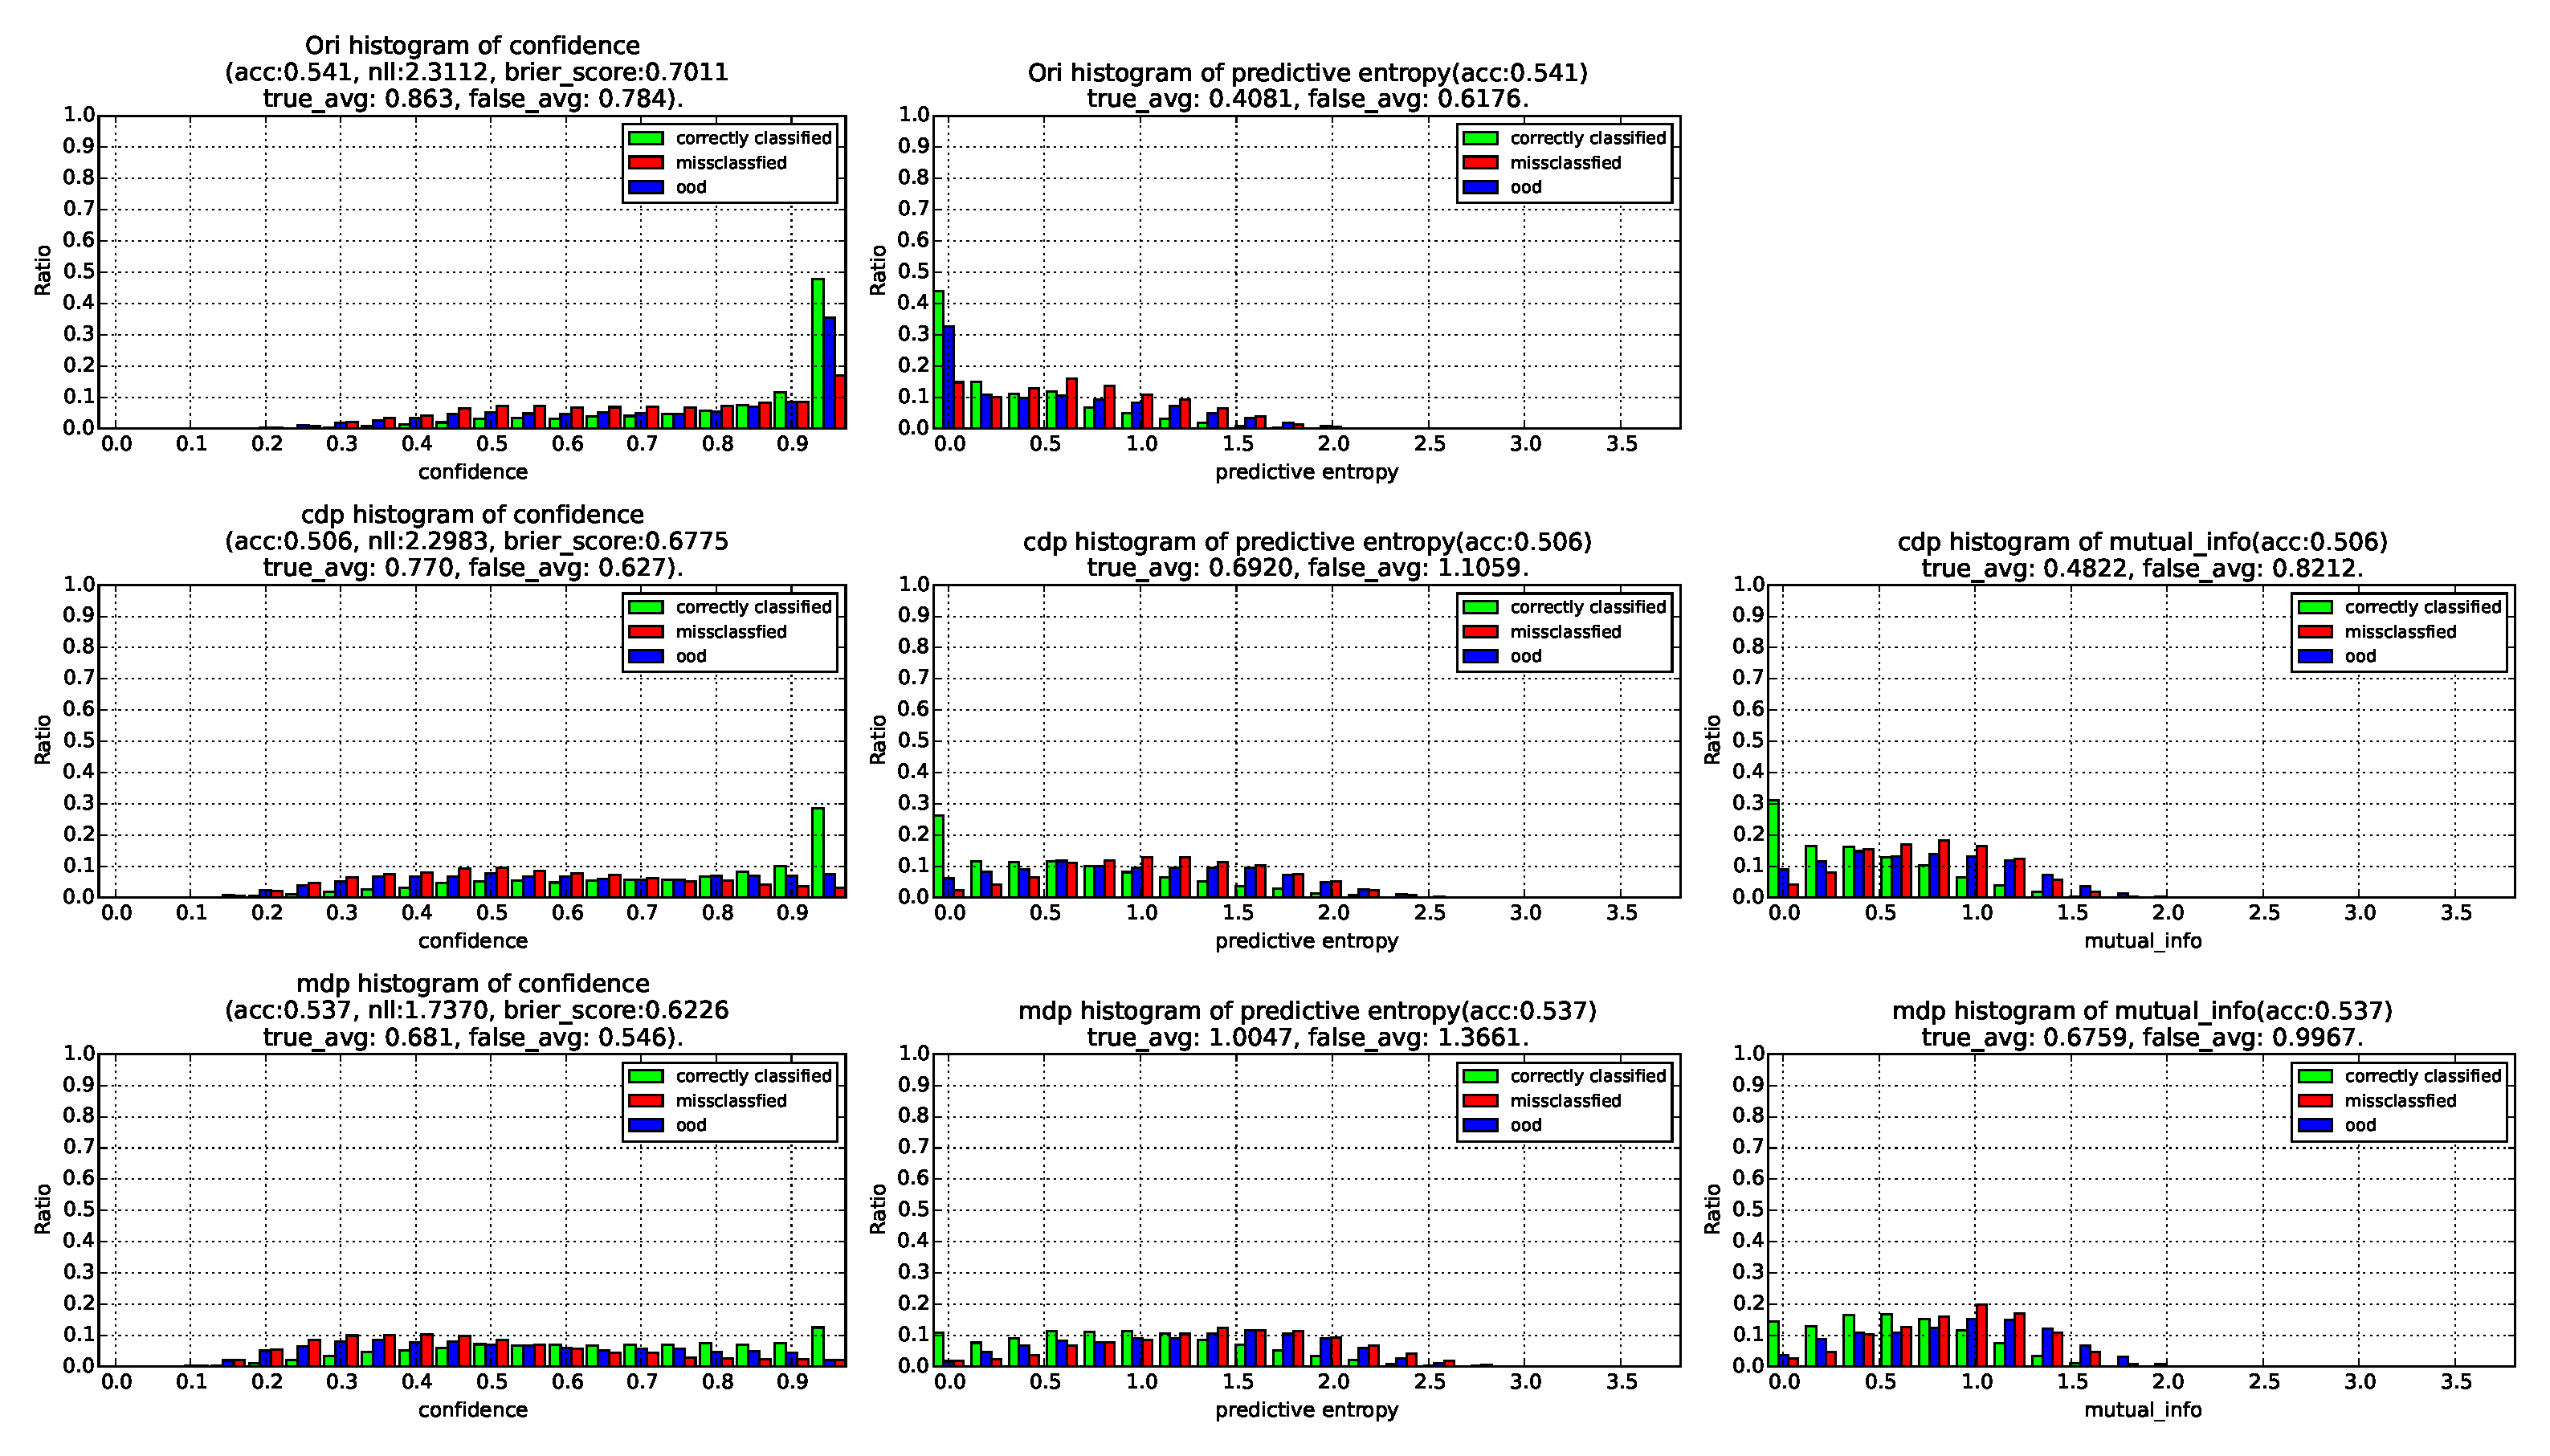
\includegraphics[height=9cm, width=16cm]{uncertainty_estimation/ablation_study/histo_froFeat_ori_cdp_mdp_ood_seed3.eps}
		\caption{Uncertainty histogram of one of three runs.}		
		\label{exp1_reliability}
	\end{center}
\end{figure}

This is Reliability diagram
\begin{figure}[H]
	\begin{center}
		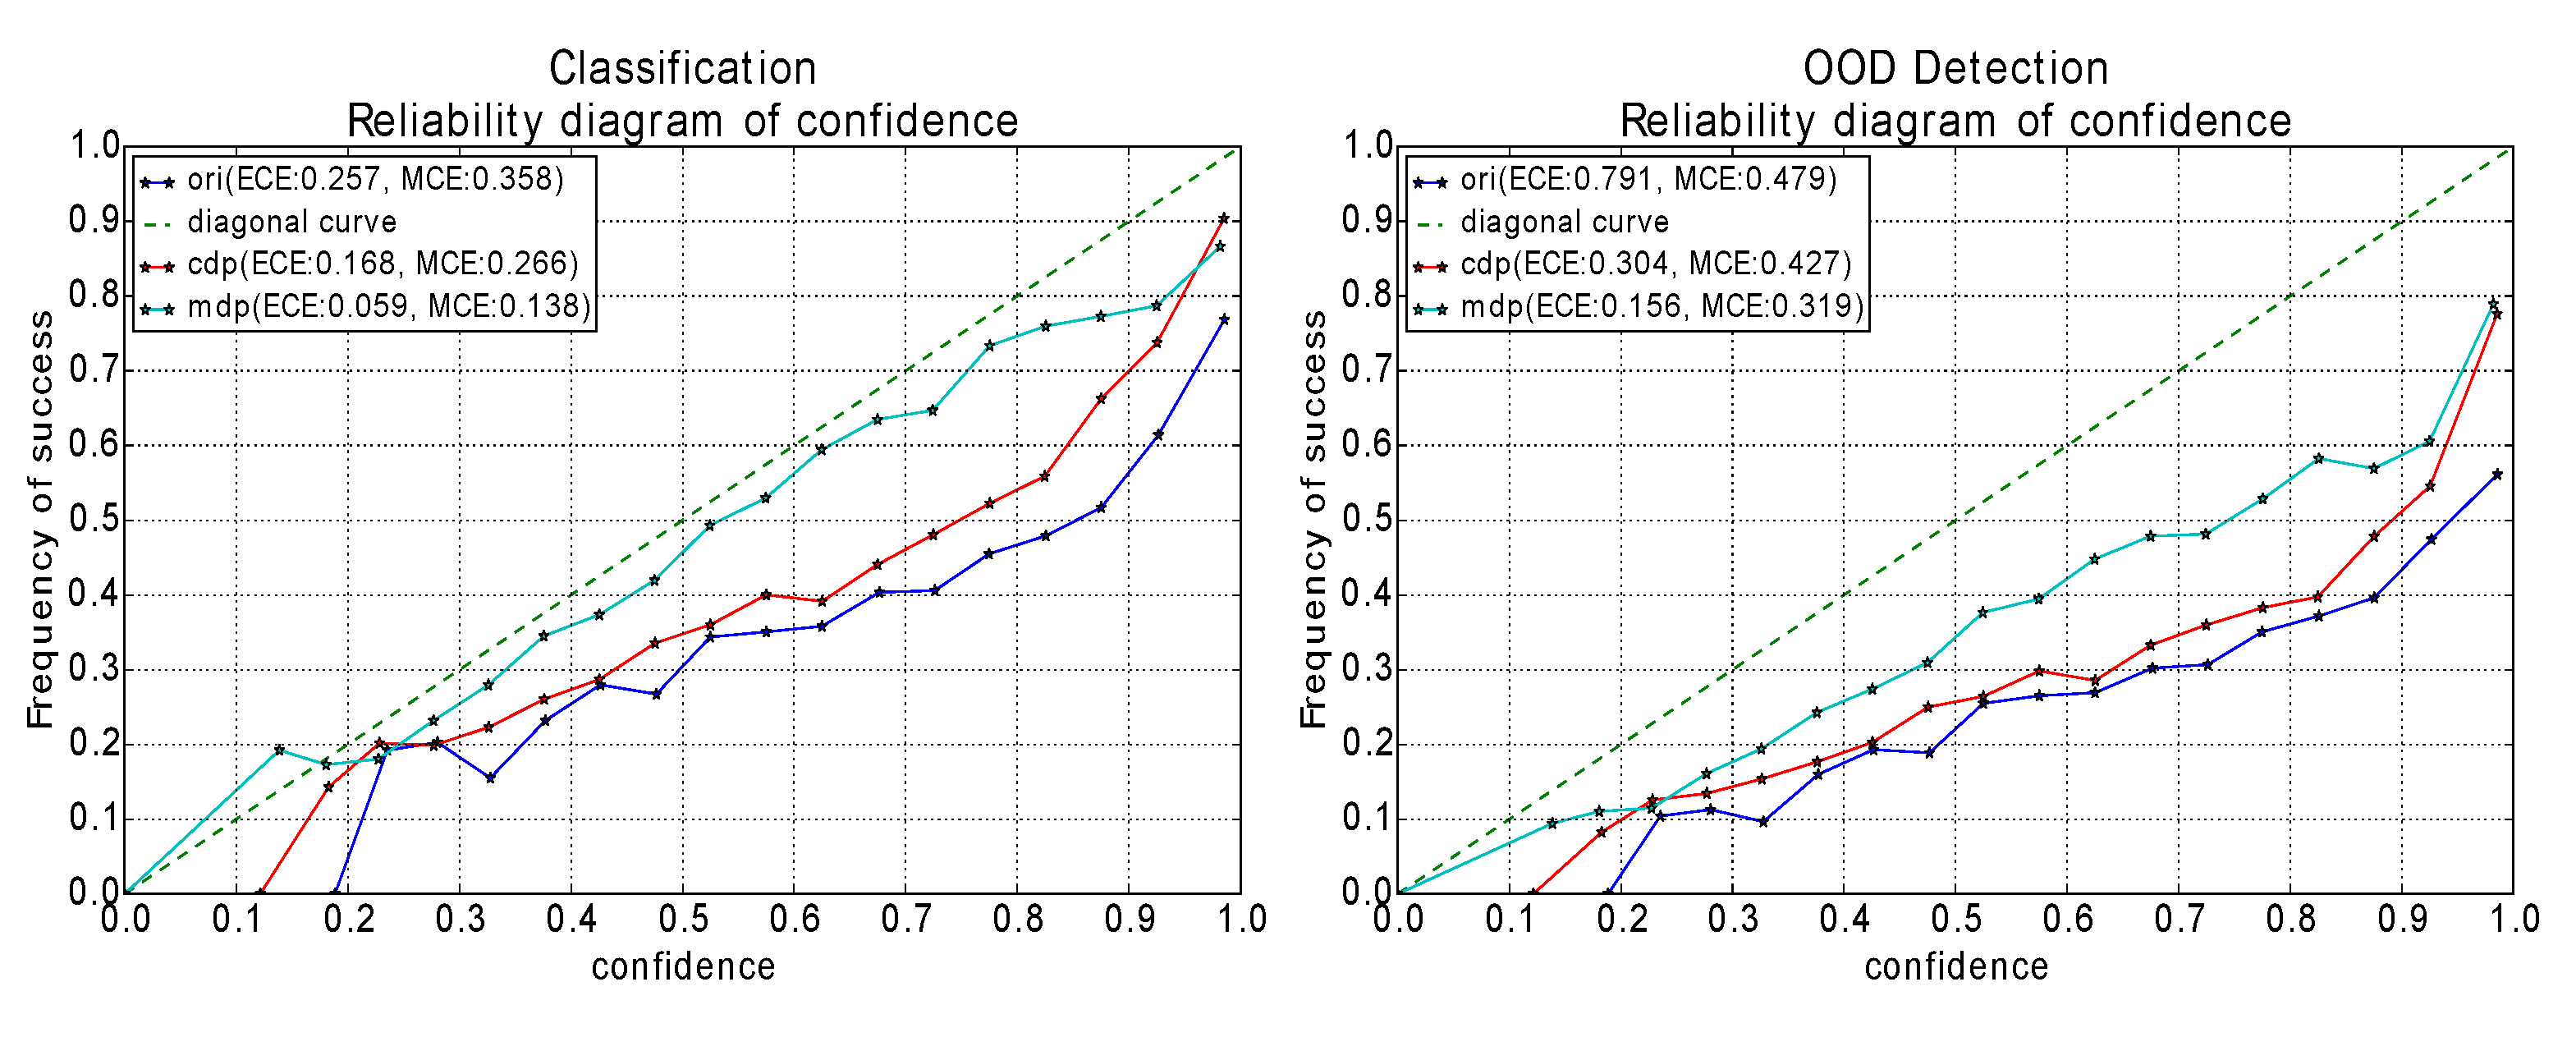
\includegraphics[height=6cm, width=16.5cm]{uncertainty_estimation/ablation_study/reliability_froFeat_ori_cdp_mdp_combined_seed3_.eps}
		\caption{Calibration curve of one of three runs.}		
		\label{exp1_reliability}
	\end{center}
\end{figure}

This is ROC and PR curve
\begin{figure}[H]
	\begin{center}
		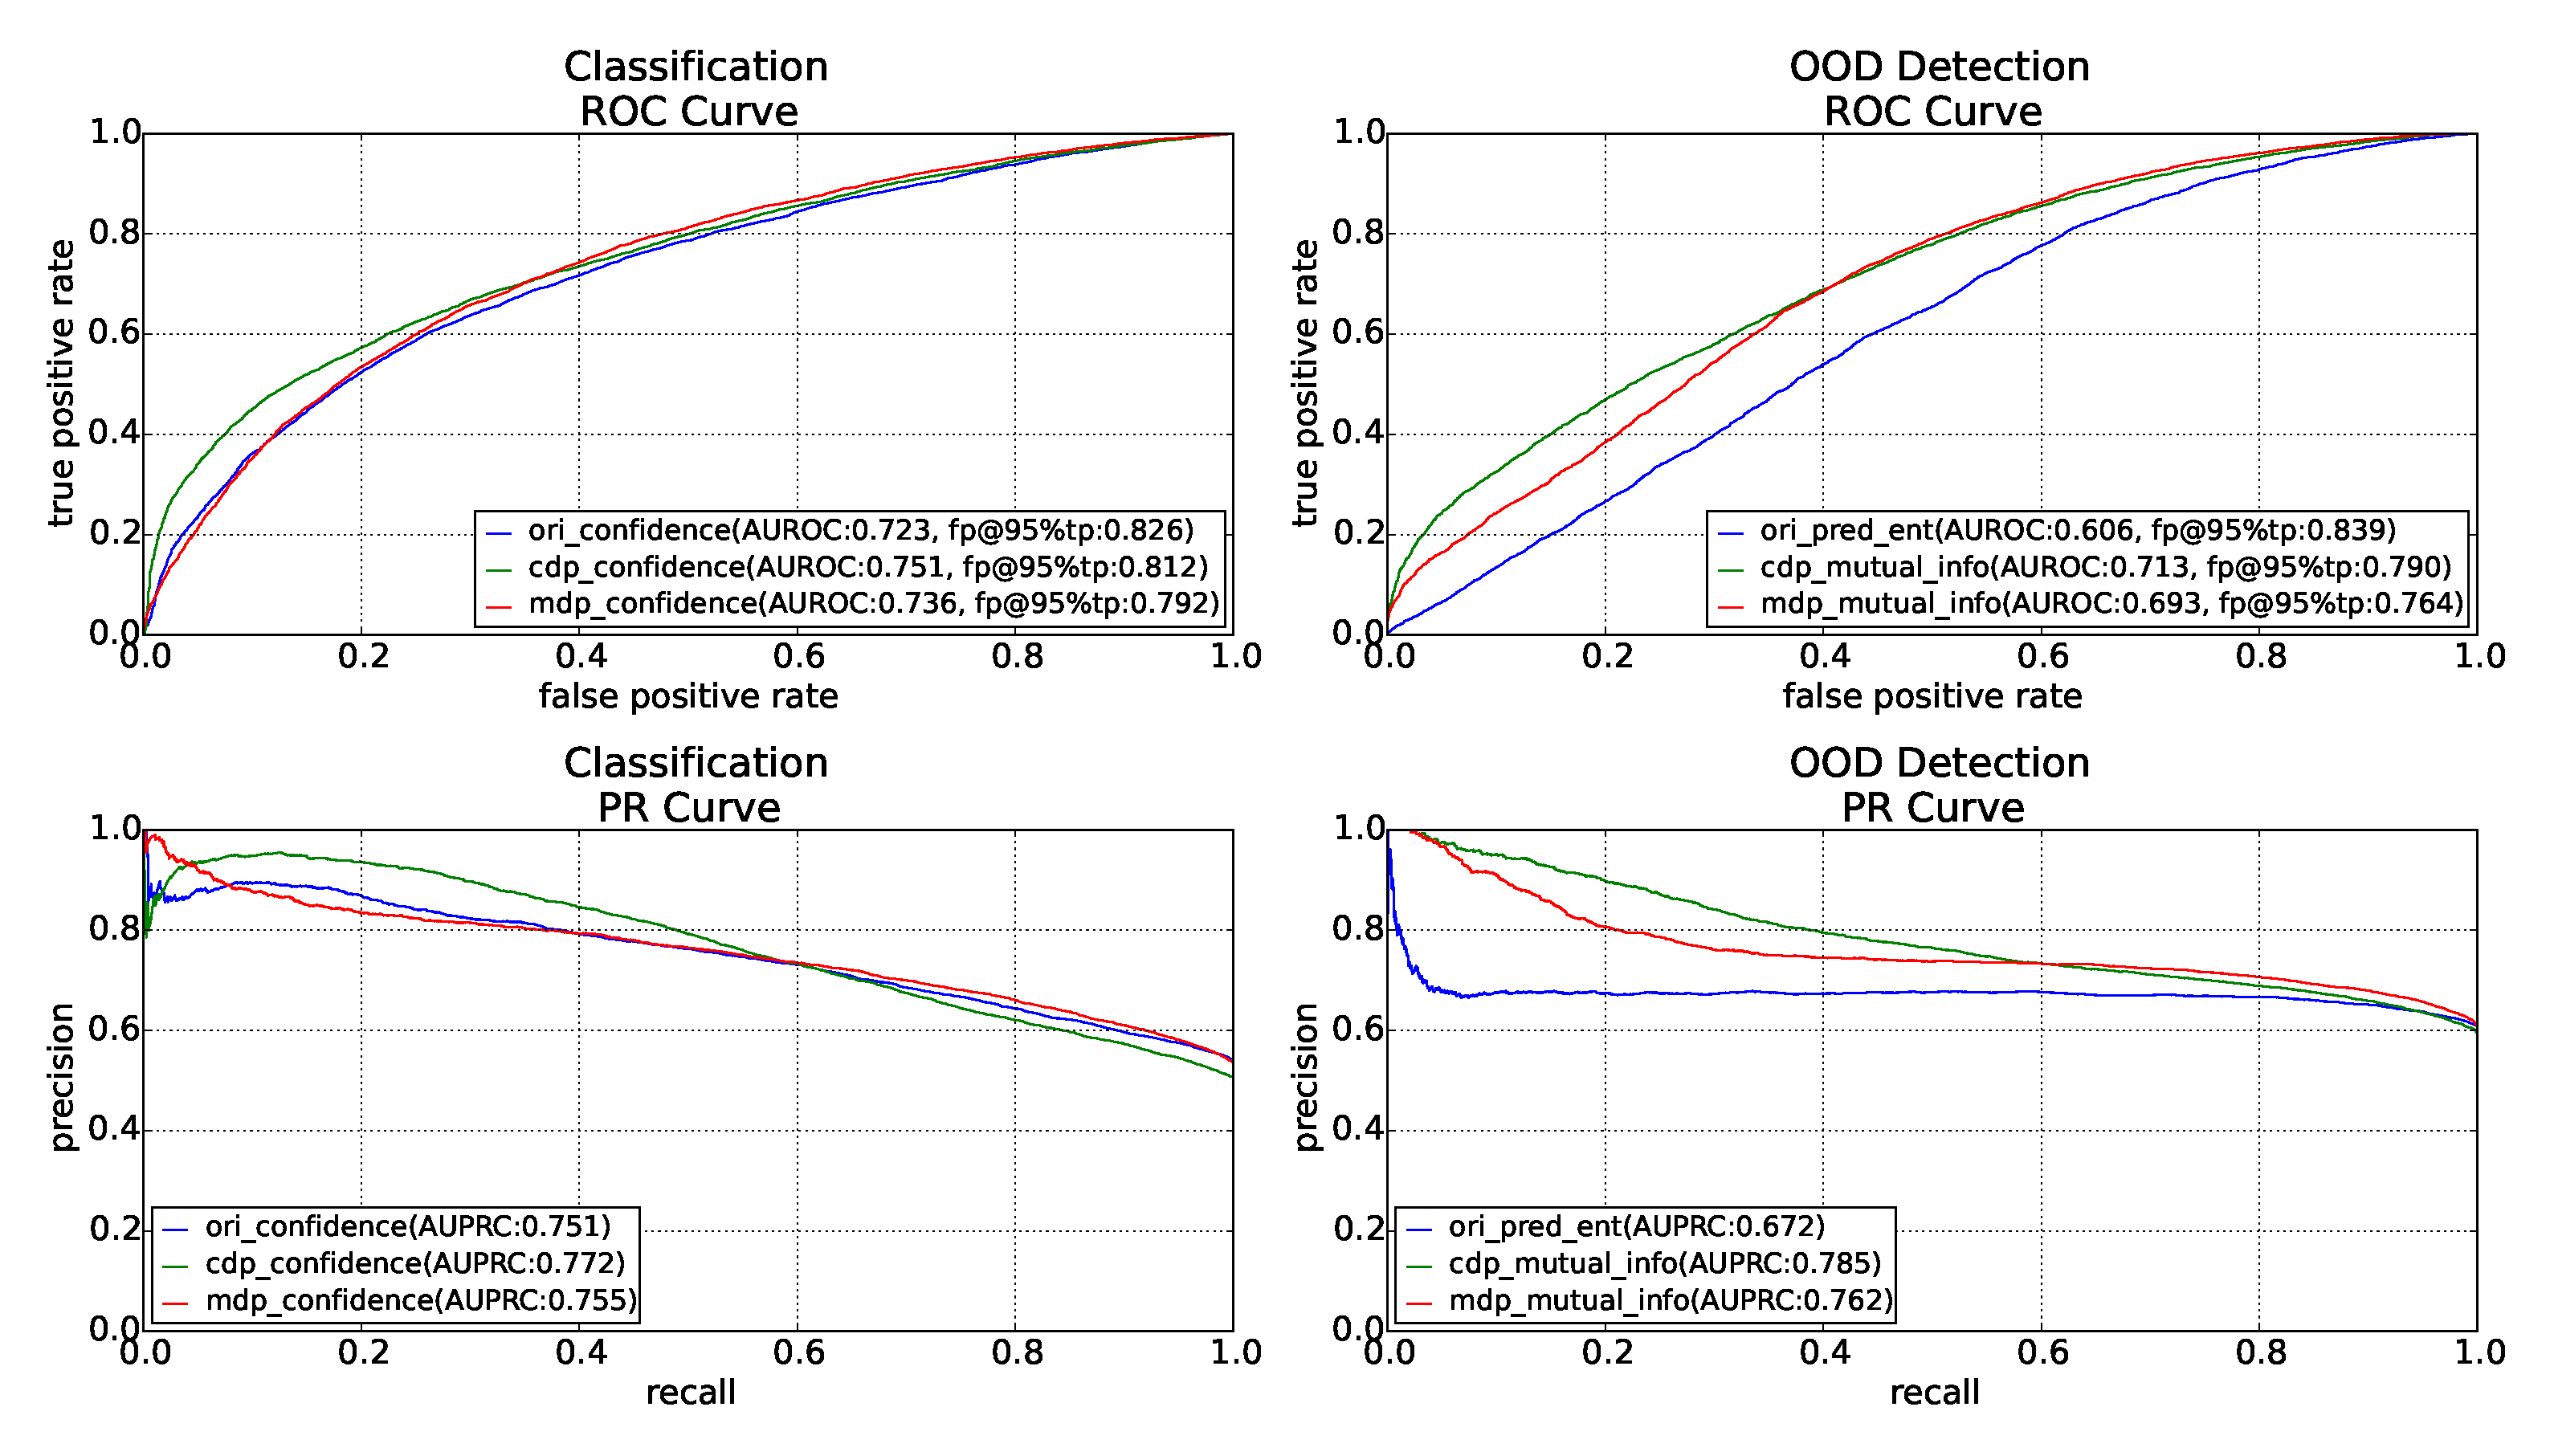
\includegraphics[height=9cm, width=16cm]{uncertainty_estimation/ablation_study/roc_pr_froFeat_ori_cdp_mdp_combined_seed3.eps}
		\caption{ROC and PR curve of one of three runs.}		
		\label{exp1_reliability}
	\end{center}
\end{figure}
\begin{table}[H]
	\centering
	\caption{results of acc, bs, nll, ece, mce, auroc, aupr}
	\begin{tabular}{|l|l|l|l|}
		\hline
		& accuracy   $\boldsymbol \uparrow$  & brier\_score $\boldsymbol \downarrow$& \begin{tabular}[c]{@{}l@{}}negative\\ log \\ likelihood $\boldsymbol \downarrow$\end{tabular} \\ \hline
		ori           &0.532$\pm$0.015 & 0.717$\pm$0.023& 2.383$\pm$0.053                                                        \\ \hline
		cdp           & 0.521$\pm$0.011&0.655$\pm$0.017 &  2.190$\pm$0.149                                                        \\ \hline
		mdp           & 0.520$\pm$0.012 &0.641$\pm$0.014 & 1.804$\pm$0.073                                                         \\ \hline
	\end{tabular}
\end{table}

\begin{table}[H]
	\centering
	% \caption{results of ece, mce, auroc, aupr}
	\begin{tabular}{|l|l|l|l|l|}
		\hline
		& \begin{tabular}[c]{@{}l@{}}expected\\ calibration\\ error(w/o. OOD/\\ w. OOD)$\boldsymbol \downarrow$\end{tabular} & \begin{tabular}[c]{@{}l@{}}maximal\\ calibration\\ error(w/o. OOD/\\ w. OOD)$\boldsymbol \downarrow$\end{tabular} & \begin{tabular}[c]{@{}l@{}}area under\\ ROC\\ (vs. Miss-\\ classified/\\ vs. OOD)$\boldsymbol \uparrow$\end{tabular} & \begin{tabular}[c]{@{}l@{}}area under\\ PR curve\\ (vs. Miss-\\ classified/\\ vs. OOD)$\boldsymbol \uparrow$\end{tabular} \\ \hline
		ori           & \begin{tabular}[c]{@{}l@{}}0.262$\pm$0.011/ \\0.793$\pm$0.012\end{tabular}                      & \begin{tabular}[c]{@{}l@{}}0.365$\pm$0.010/ \\0.491$\pm$0.013\end{tabular}                     &
		\begin{tabular}[c]{@{}l@{}}0.716$\pm$0.005/ \\0.602$\pm$0.014\end{tabular}           & \begin{tabular}[c]{@{}l@{}}0.724$\pm$0.022/ \\0.681$\pm$0.007\end{tabular}                \\ \hline
		cdp           & \begin{tabular}[c]{@{}l@{}}0.141$\pm$0.022/ \\0.270$\pm$0.037\end{tabular}                     & \begin{tabular}[c]{@{}l@{}}0.203$\pm$0.053/ \\0.359$\pm$0.056\end{tabular}                     & \begin{tabular}[c]{@{}l@{}}0.748$\pm$0.002/ \\0.712$\pm$0.006\end{tabular}           & \begin{tabular}[c]{@{}l@{}}0.770$\pm$0.002/ \\0.782$\pm$0.004\end{tabular}                \\ \hline
		
		mdp           & \begin{tabular}[c]{@{}l@{}}0.068$\pm$0.009/ \\0.158$\pm$0.006\end{tabular}                      & \begin{tabular}[c]{@{}l@{}}0.134$\pm$0.018/ \\0.311$\pm$0.008\end{tabular}                     & \begin{tabular}[c]{@{}l@{}}0.730$\pm$0.009/ \\0.674$\pm$0.014\end{tabular}           & \begin{tabular}[c]{@{}l@{}}0.749$\pm$0.009/ \\0.748$\pm$0.010\end{tabular}                \\ \hline
	\end{tabular}
\end{table}	


\section{Automatic labeling experiments}
\subsection{Experiments settings}
\subsection{Results}
\subsection{Analysis}


\section{Context-based improvement experiments}
\subsection{Experiments settings}
\subsection{Results}
\subsection{Analysis}